\documentclass[11pt,oneside]{article}

\usepackage[T1]{fontenc}
\usepackage[utf8]{inputenc}
\IfFileExists{libertinus.sty}{\usepackage{libertinus}}{\usepackage{lmodern}}
\usepackage{microtype}
\usepackage[a4paper,margin=1in]{geometry}
\usepackage{amsmath,amssymb,amsthm,mathtools,mathrsfs}
\usepackage{bm}
\usepackage{booktabs,longtable,array}
\usepackage{graphicx}
\usepackage{xcolor}
\usepackage{enumitem}
\usepackage{listings}
\usepackage{xurl}
\usepackage{hyperref}
\usepackage[nameinlink,capitalize,noabbrev]{cleveref}
\usepackage{fancyhdr}
\usepackage{caption}
\usepackage{setspace}

\hypersetup{
  colorlinks=true,
  linkcolor=blue!55!black,
  citecolor=green!35!black,
  urlcolor=blue!55!black,
  pdftitle={Legendre Polynomials in the Rvachev Up Dictionary},
  pdfauthor={Prepared for the ProveIt Fabius--Rvachev project}
}

\setlength{\parindent}{1.25em}
\setlength{\parskip}{0.25em}
\allowdisplaybreaks
\numberwithin{equation}{section}

\pagestyle{fancy}
\setlength{\headheight}{14pt}
\fancyhf{}
\fancyhead[L]{Legendre--Rvachev closed loops}
\fancyhead[R]{\thepage}
\renewcommand{\headrulewidth}{0.4pt}

\newtheorem{theorem}{Theorem}[section]
\newtheorem{proposition}[theorem]{Proposition}
\newtheorem{lemma}[theorem]{Lemma}
\newtheorem{corollary}[theorem]{Corollary}
\newtheorem{conjecture}[theorem]{Conjecture}
\newtheorem{problem}[theorem]{Problem}
\theoremstyle{definition}
\newtheorem{definition}[theorem]{Definition}
\newtheorem{example}[theorem]{Example}
\newtheorem{observation}[theorem]{Computational observation}
\theoremstyle{remark}
\newtheorem{remark}[theorem]{Remark}

\newenvironment{resultbox}[1]
{\begin{center}\begin{minipage}{0.94\textwidth}\hrule\vspace{0.45em}
\noindent\textbf{#1.}\ }{\vspace{0.45em}\hrule\end{minipage}\end{center}}

\newcommand{\Up}{\operatorname{up}}
\newcommand{\M}{M_u}
\newcommand{\Dscr}{\mathscr D_u}
\newcommand{\Lscr}{\mathscr L_u}
\newcommand{\R}{\mathbb R}
\newcommand{\C}{\mathbb C}
\newcommand{\Z}{\mathbb Z}
\newcommand{\N}{\mathbb N}
\newcommand{\E}{\mathbb E}
\newcommand{\dd}{\,\mathrm d}
\newcommand{\ii}{\mathrm i}
\newcommand{\e}{\mathrm e}
\newcommand{\sincpi}{\operatorname{sinc}_{\pi}}
\newcommand{\Span}{\operatorname{span}}
\newcommand{\diag}{\operatorname{diag}}
\newcommand{\rank}{\operatorname{rank}}
\newcommand{\tr}{\operatorname{tr}}
\newcommand{\Id}{\operatorname{Id}}
\newcommand{\ord}{\operatorname{ord}}
\newcommand{\wt}{\operatorname{wt}}
\newcommand{\abs}[1]{\left|#1\right|}
\newcommand{\norm}[1]{\left\lVert#1\right\rVert}
\newcommand{\inner}[2]{\left\langle #1,#2\right\rangle}
\newcommand{\bigO}{\mathcal O}
\newcommand{\smallo}{o}
\newcommand{\rev}{\operatorname{rev}}

\lstdefinestyle{pythonstyle}{
  language=Python,
  basicstyle=\ttfamily\small,
  keywordstyle=\bfseries,
  commentstyle=\itshape,
  showstringspaces=false,
  breaklines=true,
  frame=single,
  columns=fullflexible
}

\title{\textbf{Legendre Polynomials in the Rvachev Up Dictionary}\\[0.4em]
\large Symmetric finite synthesis, closed Fourier--Legendre loops,\\
and transmuted spectral geometry}
\author{Research report for the ProveIt Fabius--Rvachev project}
\date{29 August 2026}

\begin{document}
\maketitle

\begin{abstract}
Let $u=\Up$ denote Rvachev's compactly supported $C^\infty$ atomic function,
normalized as an even probability density on $[-1,1]$.  The repository under
study contains two ingredients that naturally point toward a closed loop: an
exact finite representation of every polynomial by shifted copies of $u$, and
the absolutely and uniformly convergent Fourier--Legendre expansion
\[
  u(x)=\sum_{n\ge0}u_nP_{2n}(x),\qquad -1\le x\le1.
\]
If
\[
  Q_n=\Dscr P_n,\qquad \Dscr=\M(D)^{-1},
\]
where $\M$ is the moment generating function of the up-law, then the required
Legendre specialization is
\[
 P_{2n}(x)=\frac1{4^n}\sum_{|k|<2\cdot4^n}
 Q_{2n}(k/4^n)u(x-k/4^n).
\]
Substitution gives an exact self-representation of $u$ by finite cancellation
blocks.  The grouped order is essential: the repeated atom coefficients do not
form an unconditional scalar series.

Beyond this specialization, the report develops several corpus-relative new
results.  The deconvolved Legendre polynomials are orthogonal for a positive
pullback inner product and diagonalize the conjugated nonlocal operator
\[
 \Lscr=-D(1-X_u^2)D,\qquad
 X_u=x-\frac{\M'(D)}{\M(D)}.
\]
This gives an operator-valued three-term recurrence, a transmuted
Christoffel--Darboux identity, exact continuous--discrete biorthogonality, a
Gram-metric projector, and a positive two-sided factorization of the even
Legendre projection kernel by up-atoms.  An exact Favard obstruction explains
why this orthogonality is not generated by an ordinary scalar weight.

A second new strand exploits reflection symmetry in the one-cell up-spline
space.  At even degree $2N$, its reflection-even part is exactly the centered
even polynomial space.  The $N+1$ central reflected pairs
\[
 \psi_{-r}(t)+\psi_{r+1}(t),\qquad r=0,\ldots,N,
\]
therefore become polynomial automatically.  Their independence is certified by
an explicit odd determinant
\[
 \det B_N=(-1)^N(C_N\sigma_N-1),\qquad
 C_N=2^{1+N(2N-1)},
\]
where
\[
 \sigma_N=[z^N]\frac{(1-z)^{2N-2}}
 {\prod_{m=1}^{2N-1}(1-z^{2^m})}.
\]
Consequently every $P_{2m}$ with $m\le N$ has a unique centrally symmetric
common-scale representation using exactly $N+1$ pair blocks.  Substitution into
the Legendre partial sum gives a new symmetric finite closed loop converging to
$u$ in every $C^r$ norm.  Exact symbolic checks, numerical experiments,
conjectures, and a fully commented Python program are included.
\end{abstract}

\tableofcontents
\newpage

\section{Scope, corpus audit, and status discipline}
\label{sec:scope}

\subsection{Audit strategy}

The recursive \texttt{docs} tree of the ProveIt Fabius-function project was
surveyed through its live manifest, directory structure, consolidated source
maps, and provenance notes.  The full text of the directly relevant current
TeX volumes was then audited, with targeted searches across adjacent live
volumes.  Files marked by the repository as byte-identical, absorbed,
superseded, or provenance-only were treated as historical witnesses rather
than mathematically independent sources.  This avoids counting editorial
copies as separate prior results.

The principal nonduplication boundaries are summarized in
\cref{tab:corpus}.  The repository's primary Fabius--Rvachev exposition and
polynomial-synthesis consolidation are cited as
\cite{ReshetnikovPrimary,ReshetnikovSynthesis}; the closest pre-existing loop
drafts are cited as \cite{ReshetnikovLoopV3,ReshetnikovLoopV4}.

\begin{table}[htbp]
\centering
\caption{Repository sources most directly relevant to this report.}
\label{tab:corpus}
\begin{tabular}{p{0.24\textwidth}p{0.31\textwidth}p{0.37\textwidth}}
\toprule
Source & Role here & Imported material or nonduplication boundary\\
\midrule
\emph{The Fabius Function and Rvachev's Up-Function}
& Primary exposition and formal-development crosswalk
& Fourier and sinc products, MGF and moments, exact Legendre coefficients,
absolute/uniform convergence, cosine series, Poisson identities\\
\addlinespace
\emph{Up Polynomial Synthesis}
& Consolidated arbitrary-polynomial theorem
& Scale classification, global/local synthesis, endpoint basis, local
dimension $d+2$, annihilator $A_d$, canonical defect, Appell--Bell--Bernoulli
calculus\\
\addlinespace
\emph{Closing the Lagrange--Legendre--Rvachev Loop} (v3)
& Closest existing loop report
& Literal Legendre atomization, grouped closure, endpoint compression,
deconvolved recurrence, factorial growth and nonflattening, one-sided kernel
factorization\\
\addlinespace
\emph{Lagrange--Rvachev Closed-Loop Report} (v4)
& Wider multiscale/Lagrange synthesis
& Scale-ladder closure, node cancellation, two-atom Appell blocks, Lambert--$W$
conditioning discussion\\
\addlinespace
Adjacent frontier volumes
& Cross-connections
& Thue--Morse products, binary partitions, inverse/sampling identities,
Lambert--$W$ asymptotics, Bell and Bernoulli polynomial machinery\\
\bottomrule
\end{tabular}
\end{table}

One recent loop draft already contains the literal formula for $P_{2n}$ and
its substitution into the Legendre expansion.  This report therefore marks
that operation as imported.  Its new work begins with the pure Legendre
transmutation, the parity-compressed local space, the central-pair determinant,
the symmetric minimal-pair loop, the exact Gram geometry, and the two-sided
kernel factorization.

\subsection{Meaning of ``new''}

Throughout, ``new'' means \emph{not found in the audited repository snapshot
and not encountered in the targeted literature search used for this report}.
It is not an unqualified claim of global priority.  Imported statements are
identified, proofs are supplied for new theorems, numerical observations are
not promoted to theorems, and conjectures are explicitly labeled.

\begin{resultbox}{Contribution map}
The report separates four levels of closure:
\begin{enumerate}[leftmargin=1.8em,itemsep=0.2em]
\item the imported literal shift-only Legendre atomization and grouped infinite
loop;
\item a new pullback-orthogonal, probabilistic, and nonlocal
Sturm--Liouville interpretation of the deconvolved Legendre family;
\item new exact Gram, biorthogonal, projector, and tensor-kernel identities at
every finite cutoff;
\item a new centrally symmetric $N+1$-pair basis with an odd $q$-product
determinant, yielding a common-scale loop convergent in $C^\infty$.
\end{enumerate}
\end{resultbox}

\section{The up-function, its probability law, and Appell calculus}
\label{sec:background}

\subsection{Normalization and Fourier product}

Let $u=\Up$ be the even $C^\infty$ function supported on $[-1,1]$, normalized
by
\[
 u(0)=1,\qquad \int_{-1}^{1}u(x)\dd x=1.
\]
With the Fourier convention
\[
 \widehat f(\xi)=\int_{\R}f(x)\e^{-2\pi\ii\xi x}\dd x,
\]
its transform is
\begin{equation}
 \widehat u(\xi)=\prod_{j=0}^{\infty}
 \sincpi\!\left(\frac{\xi}{2^j}\right),
 \qquad \sincpi(t)=\frac{\sin(\pi t)}{\pi t}.
 \label{eq:fourier-product}
\end{equation}
At a nonzero integer $m$,
\begin{equation}
 \ord_{\xi=m}\widehat u(\xi)=1+\nu_2(m),
 \label{eq:zero-order}
\end{equation}
where $\nu_2$ is the dyadic valuation.  This zero multiplicity is the source
of the sharp degree-$d$ reproduction scale $2^d$.

On $[0,1]$, the Fabius function is related by
\begin{equation}
 F(t)=u(t-1),
 \label{eq:F-up}
\end{equation}
with the standard continuation supplied by its functional equations.  Dyadic
values of $F$ therefore encode exact moments and Legendre coefficients of $u$.
The original nowhere-analytic $C^\infty$ example goes back to Fabius
\cite{Fabius1966}.

\subsection{Probability representation and moment generating function}

Let $V_1,V_2,\ldots$ be independent uniform random variables on $[-1,1]$ and
put
\begin{equation}
 Z=\sum_{j=1}^{\infty}2^{-j}V_j.
 \label{eq:random-series}
\end{equation}
Then $Z$ has density $u$.  Its moment generating function is
\begin{equation}
 \M(z)=\E\e^{zZ}
 =\prod_{j=1}^{\infty}\frac{\sinh(z/2^j)}{z/2^j}
 =\sum_{r=0}^{\infty}\mu_r\frac{z^r}{r!}.
 \label{eq:mgf}
\end{equation}
The law is symmetric, so odd moments vanish.  The first even moments are
\begin{equation}
 \mu_0=1,\qquad \mu_2=\frac19,\qquad
 \mu_4=\frac{19}{675},\qquad
 \mu_6=\frac{583}{59535}.
 \label{eq:moments}
\end{equation}
Writing
\[
 \log\M(z)=\sum_{r\ge1}\kappa_r\frac{z^r}{r!},
\]
one obtains
\begin{equation}
 \kappa_{2r}=\frac{B_{2r}}{2r(1-4^{-r})},
 \qquad \kappa_{2r+1}=0.
 \label{eq:cumulants}
\end{equation}
Thus the up-law is tied directly to Bernoulli numbers.

\subsection{Reciprocal MGF, Bell polynomials, and deconvolution}

Define rational coefficients $\gamma_r$ by
\begin{equation}
 \frac1{\M(z)}=\sum_{r=0}^{\infty}\gamma_r\frac{z^r}{r!}.
 \label{eq:gamma-def}
\end{equation}
In terms of complete Bell polynomials,
\begin{equation}
 \gamma_r=Y_r(-\kappa_1,\ldots,-\kappa_r).
 \label{eq:gamma-bell}
\end{equation}
The first nonzero values are
\begin{equation}
 \gamma_2=-\frac19,\quad
 \gamma_4=\frac{31}{675},\quad
 \gamma_6=-\frac{2347}{59535},\quad
 \gamma_8=\frac{1904369}{32531625}.
 \label{eq:gamma-values}
\end{equation}
The finite-on-polynomials deconvolution operator is
\begin{equation}
 \Dscr=\M(D)^{-1}=\sum_{r\ge0}\gamma_r\frac{D^r}{r!},
 \label{eq:deconvolution}
\end{equation}
with inverse
\begin{equation}
 \M(D)=\sum_{r\ge0}\mu_r\frac{D^r}{r!}.
 \label{eq:moment-operator}
\end{equation}
The monomial images
\begin{equation}
 A_n(x)=\Dscr x^n=\sum_{r=0}^{n}\binom nr\gamma_r x^{n-r}
 \label{eq:appell-polys}
\end{equation}
form an Appell family with generating function
\begin{equation}
 \sum_{n\ge0}A_n(x)\frac{z^n}{n!}=\frac{\e^{xz}}{\M(z)}.
 \label{eq:appell-egf}
\end{equation}

The probability representation supplies a useful interpretation.  For every
polynomial $f$,
\begin{equation}
 (\M(D)f)(x)=\E f(x+Z).
 \label{eq:translation-expectation}
\end{equation}
Hence $q=\Dscr p$ is characterized by the exact deconvolution equation
\begin{equation}
 \E q(x+Z)=p(x).
 \label{eq:prob-deconv}
\end{equation}

\subsection{Thue--Morse and q-integer products}

Let $\varepsilon_j=(-1)^{\wt(j)}$ be the Thue--Morse signs.  The finite Prouhet
product is
\begin{equation}
 \Theta_m(z)=\prod_{j=0}^{m-1}(1-z^{2^j})
 =\sum_{j=0}^{2^m-1}\varepsilon_jz^j.
 \label{eq:thue-morse-product}
\end{equation}
The annihilator governing local up-atom dependencies is
\begin{equation}
 \mathcal A_d(z)=\prod_{m=1}^{d}[2^m]_z
 =\prod_{m=1}^{d}\frac{1-z^{2^m}}{1-z}
 =\prod_{\ell=1}^{d}(1+z^{2^{\ell-1}})^{d-\ell+1}.
 \label{eq:annihilator}
\end{equation}
It is monic and palindromic, with
\begin{equation}
 R_d:=\deg\mathcal A_d=2^{d+1}-d-2,
 \qquad \mathcal A_d(1)=2^{d(d+1)/2}.
 \label{eq:annihilator-data}
\end{equation}
The determinant in \cref{sec:central} will involve a reciprocal of this
$q$-product and therefore restricted binary partitions.

\section{Imported arbitrary-polynomial synthesis}
\label{sec:poly-synthesis}

\subsection{Global common-scale formula}

Let $p\in\Pi_d$, where $\Pi_d$ denotes the real polynomials of degree at most
$d$, and set
\begin{equation}
 M=2^d,\qquad q=\Dscr p.
 \label{eq:physical-q}
\end{equation}
The physical-lattice form of the repository's synthesis theorem is as follows
\cite{ReshetnikovSynthesis}.

\begin{theorem}[Imported exact polynomial synthesis]
\label{thm:physical-synthesis}
For every $p\in\Pi_d$,
\begin{equation}
 \boxed{
 p(x)=\frac1M\sum_{k\in\Z}q(k/M)u(x-k/M),\qquad x\in\R.}
 \label{eq:physical-synthesis}
\end{equation}
The sum is locally finite.  On $[-1,1]$ it reduces to
\begin{equation}
 p(x)=\frac1M\sum_{|k|<2M}q(k/M)u(x-k/M).
 \label{eq:finite-physical}
\end{equation}
\end{theorem}

\begin{proof}[Scaling check]
The normalized-cell formula in the repository is
\[
 P(t)=\frac1M\sum_{k\in\Z}Q(k)u\!\left(\frac{t-k}{M}\right),
 \qquad Q=\M(MD)^{-1}P.
\]
Apply it to $P(t)=p(t/M)$ and put $t=Mx$.  Since $D_t=M^{-1}D_x$,
$Q(k)=\Dscr p(k/M)$, which gives \eqref{eq:physical-synthesis}.  In the
Fourier proof, nonzero aliases contain derivatives through degree $d$ of
$\widehat u(M\xi)$ at integer frequencies; \eqref{eq:zero-order} makes them
vanish.  Compact support gives local finiteness.  On $[-1,1]$, centers with
$|k|\ge2M$ meet only the exterior or a flat support endpoint.
\end{proof}

\subsection{Sharp scale, local dimension, and endpoint basis}

For the normalized one-cell atoms
\begin{equation}
 \psi_k(t)=\frac1M u\!\left(\frac{t-k}{M}\right),
 \qquad 0\le t\le1,
 \label{eq:cell-atoms}
\end{equation}
only the $2M$ centers $-M+1\le k\le M$ are active.  The repository proves that
the integer-translate system at ratio $\rho\in\N$ has exact polynomial
reproduction order $\nu_2(\rho)$.  Thus $M=2^d$ is the smallest integer ratio
reproducing all of $\Pi_d$.

Set
\begin{equation}
 V_d=\Span\{\psi_k|_{[0,1]}:-M+1\le k\le M\}.
 \label{eq:Vd}
\end{equation}
Then
\begin{equation}
 \dim V_d=d+2,\qquad V_d\cap\R[t]=\Pi_d.
 \label{eq:local-dimension}
\end{equation}
The $d+2$ rightmost atoms
\begin{equation}
 \mathcal B_d=\{\psi_k|_{[0,1]}:M-d-1\le k\le M\}
 \label{eq:endpoint-basis}
\end{equation}
form a basis of $V_d$.  Any degree-$d$ polynomial can therefore be compressed
from exponentially many literal lattice atoms to $d+2$ atoms, although the
resulting signed coefficients may be very large.

\subsection{The one-dimensional defect}

The quotient $V_d/\Pi_d$ is one-dimensional.  A canonical representative is
\begin{equation}
 \mathcal D_d(t)=t^{d+1}+\mathcal E_d(t),
 \label{eq:defect}
\end{equation}
where
\begin{equation}
 \mathcal E_d(t)=-\frac{(d+1)!}{(2\pi\ii)^{d+1}}
 \sum_{\substack{n\in\Z\\ n\ \mathrm{odd}}}
 \frac{\widehat u(n/2)}{n^{d+1}}\e^{2\pi\ii nt}.
 \label{eq:defect-series}
\end{equation}
Thus
\begin{equation}
 V_d=\Pi_d\oplus\Span\{\mathcal D_d\}.
 \label{eq:defect-split}
\end{equation}
For odd $d$, $\mathcal E_d$ is a cosine series; for even $d$, it is a sine
series.  This parity fact drives the central-pair construction.

\section{Explicit Legendre specialization}
\label{sec:legendre-specialization}

\subsection{Deconvolved Legendre polynomials}

Let $P_n$ be normalized by $P_n(1)=1$ and define
\begin{equation}
 Q_n(x)=\Dscr P_n(x).
 \label{eq:Qn-def}
\end{equation}
Because $\Dscr$ is even, $Q_n$ has the same parity as $P_n$.  The standard
coefficient formula
\begin{equation}
 P_{2n}(x)=\sum_{j=0}^{n}a_{n,j}x^{2n-2j},\qquad
 a_{n,j}=\frac{(-1)^j}{2^{2n}}
 \frac{(4n-2j)!}{j!(2n-j)!(2n-2j)!}
 \label{eq:P-even-coeff}
\end{equation}
gives the explicit Bell--Bernoulli form
\begin{equation}
 \boxed{
 Q_{2n}(x)=\sum_{j=0}^{n}a_{n,j}
 \sum_{r=0}^{n-j}\binom{2n-2j}{2r}\gamma_{2r}
 x^{2n-2j-2r}.}
 \label{eq:Q-even-explicit}
\end{equation}
All coefficients are rational.  The first examples are
\begin{align}
 Q_0(x)&=1,\nonumber\\
 Q_2(x)&=\frac{9x^2-4}{6},\label{eq:Q2}\\
 Q_4(x)&=\frac{4725x^4-7200x^2+1072}{1080},\nonumber\\
 Q_6(x)&=\frac{654885x^6-1984500x^4+1344168x^2-114080}{45360}.
 \label{eq:Qexamples}
\end{align}
The probabilistic characterization \eqref{eq:prob-deconv} becomes
\begin{equation}
 \E Q_n(x+Z)=P_n(x).
 \label{eq:Q-probability}
\end{equation}

\subsection{Finite shift-only representation}

\begin{theorem}[Literal Legendre-to-up transform; imported specialization]
\label{thm:literal-legendre}
Let $M_n=4^n$.  For every $n\ge0$ and $-1\le x\le1$,
\begin{equation}
 \boxed{
 P_{2n}(x)=\frac1{M_n}\sum_{|k|<2M_n}
 Q_{2n}(k/M_n)u(x-k/M_n).}
 \label{eq:literal-legendre}
\end{equation}
Equivalently,
\begin{equation}
 P_{2n}(x)=\frac1{M_n}\left[
 Q_{2n}(0)u(x)+\sum_{k=1}^{2M_n-1}Q_{2n}(k/M_n)
 \bigl(u(x-k/M_n)+u(x+k/M_n)\bigr)\right].
 \label{eq:literal-legendre-parity}
\end{equation}
\end{theorem}

\begin{proof}
Apply \cref{thm:physical-synthesis} with degree $d=2n$, so
$M=2^{2n}=4^n$, and $q=Q_{2n}$.  Pair $k$ and $-k$ using the evenness of both
$Q_{2n}$ and $u$.
\end{proof}

\begin{example}[A completely explicit formula for $P_2$]
Since $M_1=4$ and \eqref{eq:Q2} holds,
\begin{equation}
 \boxed{
 P_2(x)=\frac1{384}\left[-64u(x)+
 \sum_{k=1}^{7}(9k^2-64)\bigl(u(x-k/4)+u(x+k/4)\bigr)\right].}
 \label{eq:P2-literal}
\end{equation}
This is a finite linear combination of literal translates of the undilated
up-function.
\end{example}

The odd family has the analogous antisymmetric formula.  With
$M=2^{2n+1}$,
\begin{equation}
 P_{2n+1}(x)=\frac1M\sum_{k=1}^{2M-1}Q_{2n+1}(k/M)
 \bigl(u(x-k/M)-u(x+k/M)\bigr).
 \label{eq:odd-literal}
\end{equation}

\subsection{Endpoint compression}

Mapping $t=(x+1)/2$ and applying the endpoint basis at degree $2n$ gives
unique rational coefficients $b_{n,k}$, $M_n-2n-1\le k\le M_n$, such that
\begin{equation}
 P_{2n}(x)=\frac1{M_n}
 \sum_{k=M_n-2n-1}^{M_n}b_{n,k}
 u\!\left(\frac{x+1-2k}{2M_n}\right).
 \label{eq:endpoint-legendre}
\end{equation}
This uses $2n+2$ atoms rather than $4M_n-1$ literal shifts, but its centers
cluster near one endpoint.  The central construction in \cref{sec:central}
will retain the same raw atom count while enforcing reflection symmetry.

\section{The canonical Fourier--Legendre expansion and first closed loop}
\label{sec:first-loop}

\subsection{Exact coefficients}

Evenness gives
\begin{equation}
 u(x)=\sum_{n=0}^{\infty}u_nP_{2n}(x),\qquad
 u_n=\frac{4n+1}{2}\int_{-1}^{1}u(x)P_{2n}(x)\dd x.
 \label{eq:legendre-series}
\end{equation}
The repository proves absolute and uniform convergence and supplies the exact
Fabius formula \cite{ReshetnikovPrimary}
\begin{align}
 u_n={}&4^{-n}(4n+1)\sum_{k=0}^{n}(-1)^{n+k}
 \binom{2n}{n+k}\binom{2n+2k}{2n}\notag\\
 &\hspace{4em}\times(2k)!\,2^{\binom{2k+1}{2}}F(2^{-2k-1}).
 \label{eq:un-fabius}
\end{align}
The first values are
\begin{equation}
 \begin{split}
 u_0&=\frac12,\quad u_1=-\frac56,\quad u_2=\frac{11}{30},
 \quad u_3=\frac{143}{5670},\\
 u_4&=-\frac{7291}{85050},\quad u_5=\frac{99137}{2485890},
 \quad u_6=-\frac{5726162257}{213774110550}.
 \end{split}
 \label{eq:first-un}
\end{equation}

\subsection{Termwise closure}

Substituting \eqref{eq:literal-legendre} into \eqref{eq:legendre-series}
gives the requested loop.

\begin{theorem}[Blockwise Legendre--Rvachev closed loop; imported]
\label{thm:block-loop}
For $-1\le x\le1$,
\begin{equation}
 \boxed{
 u(x)=\sum_{n=0}^{\infty}\frac{u_n}{4^n}
 \sum_{|k|<2\cdot4^n}Q_{2n}(k/4^n)u(x-k/4^n).}
 \label{eq:block-loop}
\end{equation}
The outer series converges absolutely and uniformly when each finite inner sum
is retained as one block.
\end{theorem}

\begin{proof}
The inner sum, including $4^{-n}$, is exactly $P_{2n}(x)$.  Hence the $n$th
block is $u_nP_{2n}(x)$.  Since $\norm{P_m}_{\infty}\le1$ and
$\sum_n|u_n|<\infty$, the Weierstrass test applies.
\end{proof}

The parity-compressed form is
\begin{align}
 u(x)=\sum_{n=0}^{\infty}\frac{u_n}{4^n}\Bigg[&Q_{2n}(0)u(x)\notag\\
 &+\sum_{k=1}^{2\cdot4^n-1}Q_{2n}(k/4^n)
 \bigl(u(x-k/4^n)+u(x+k/4^n)\bigr)\Bigg].
 \label{eq:block-loop-parity}
\end{align}

\subsection{One common lattice per partial sum}

Let
\begin{equation}
 S_N(x)=\sum_{n=0}^{N}u_nP_{2n}(x),\qquad
 C_N(x)=\Dscr S_N(x)=\sum_{n=0}^{N}u_nQ_{2n}(x).
 \label{eq:SN-CN}
\end{equation}
Since $S_N$ has degree $2N$, the common lattice $M=4^N$ gives
\begin{equation}
 S_N(x)=\frac1{4^N}\sum_{|k|<2\cdot4^N}
 C_N(k/4^N)u(x-k/4^N).
 \label{eq:fixed-lattice-loop}
\end{equation}
Every coefficient is rational.  Endpoint compression gives the same partial
sum with $2N+2$ atoms.

\subsection{Why grouping is essential}

The coefficient of the repeated central atom $u(x)$ in the $n$th literal block
is
\begin{equation}
 \beta_n=\frac{u_nQ_{2n}(0)}{4^n}.
 \label{eq:central-beta}
\end{equation}
The audited loop report proves
\begin{equation}
 \limsup_{n\to\infty}|\beta_n|=\infty,
 \label{eq:nonflattening}
\end{equation}
using the factorial asymptotic
\begin{equation}
 Q_{2n}(0)=\frac{2(-1)^n}{C}
 \frac{(4n)!}{(2n)!(4\pi)^{2n}}
 \left(1+\frac{2\pi^2}{4n-1}+\bigO(n^{-2})\right),
 \label{eq:Q0-asymptotic}
\end{equation}
where
\[
 C=\M(\pi\ii)=\prod_{j\ge1}\frac{\sin(\pi/2^j)}{\pi/2^j}.
\]
Thus \eqref{eq:block-loop} is a convergent series of exact cancellation
blocks, not an unconditionally convergent series indexed by individual atoms.

\section{A hidden orthogonal family: pullback Legendre geometry}
\label{sec:pullback}

The operator $\Dscr$ becomes rapidly ill-conditioned with degree, but on every
fixed polynomial space it is triangular with unit diagonal and hence
invertible.  This permits a finite-dimensional Hilbert geometry in which the
$Q_n$ are genuinely orthogonal.

\subsection{Pullback inner product and probabilistic form}

Put
\begin{equation}
 T=\M(D),\qquad A=T^{-1}=\Dscr.
 \label{eq:T-A}
\end{equation}
For polynomials define
\begin{equation}
 \inner{f}{g}_u=\int_{-1}^{1}(Tf)(x)(Tg)(x)\dd x.
 \label{eq:pullback-inner}
\end{equation}
Since $T$ is injective on polynomials, this is positive definite.  If $Z_1,Z_2$
are independent copies of \eqref{eq:random-series}, then
\begin{equation}
 \inner{f}{g}_u
 =\int_{-1}^{1}\E f(x+Z_1)\,\E g(x+Z_2)\dd x.
 \label{eq:pullback-probabilistic}
\end{equation}

\begin{theorem}[Pullback orthogonality; new]
\label{thm:pullback-orthogonality}
The deconvolved Legendre polynomials satisfy
\begin{equation}
 \boxed{
 \inner{Q_m}{Q_n}_u=h_n\delta_{mn},\qquad
 h_n=\frac{2}{2n+1}.}
 \label{eq:Q-orthogonality}
\end{equation}
Consequently $\{Q_0,\ldots,Q_d\}$ is an orthogonal basis of $\Pi_d$ for
$\inner{\cdot}{\cdot}_u$.
\end{theorem}

\begin{proof}
By definition $TQ_n=P_n$, so
\[
 \inner{Q_m}{Q_n}_u=\int_{-1}^{1}P_mP_n
 =\frac{2}{2n+1}\delta_{mn}.
\]
Triangularity of $A$ preserves degree and leading coefficient, hence the basis
claim.
\end{proof}

The inner product is explicitly derivative-coupled:
\begin{equation}
 Tf=f+\frac1{18}f''+\frac{19}{16200}f^{(4)}
 +\frac{583}{42865200}f^{(6)}+\cdots,
 \label{eq:T-expansion}
\end{equation}
with termination on each polynomial.

\begin{proposition}[No scalar-weight realization; new]
\label{prop:no-scalar-weight}
The pullback inner product cannot be represented in the form
\[
 \inner{f}{g}_u=\int f(x)g(x)\dd\rho(x)
\]
for any finite signed measure $\rho$ having all polynomial moments.
\end{proposition}

\begin{proof}
Multiplication by $x$ is symmetric for every scalar moment form.  Here
$Tx=x$ and $T(x^2)=x^2+\mu_2=x^2+1/9$, so
\[
 \inner{x}{x}_u=\int_{-1}^{1}x^2\dd x=\frac23,
 \qquad
 \inner{1}{x^2}_u=\int_{-1}^{1}\left(x^2+\frac19\right)\dd x=\frac89.
\]
The two quantities differ, proving the claim.
\end{proof}

There is also an exact Favard obstruction.  Let $\widehat Q_n$ be the monic
normalization of $Q_n$.  Direct calculation gives
\begin{align}
 \widehat Q_2&=x^2-\frac49,
 &\widehat Q_3&=x^3-\frac{14}{15}x,\notag\\
 \widehat Q_4&=x^4-\frac{32}{21}x^2+\frac{1072}{4725}.
 \label{eq:monic-Q}
\end{align}
Hence
\begin{equation}
 \boxed{
 \widehat Q_4=x\widehat Q_3-\frac{62}{105}\widehat Q_2
 -\frac{8}{225}\widehat Q_0.}
 \label{eq:favard-obstruction}
\end{equation}
A monic parity-alternating scalar orthogonal sequence would satisfy
$\widehat Q_{n+1}=x\widehat Q_n-\lambda_n\widehat Q_{n-1}$ by Favard's
theorem \cite{Szego}.  The nonzero $\widehat Q_0$ term in
\eqref{eq:favard-obstruction} rules this out for the entire $Q_n$ family,
even for an indefinite quasi-definite scalar functional.  The correct
orthogonality is operator-valued, not weighted-scalar.

\subsection{Transmuted Rodrigues formula and recurrence}

Since $A$ commutes with $D$, Rodrigues' formula becomes
\begin{equation}
 Q_n(x)=\frac1{2^nn!}D^n\left[A(x^2-1)^n\right].
 \label{eq:Q-Rodrigues}
\end{equation}
The bracket means that the differential operator $A=\M(D)^{-1}$ acts on the
polynomial seed.

To transport multiplication by $x$, use $f(D)x=xf(D)+f'(D)$.  Define
\begin{equation}
 X_u=AxT=x-\frac{\M'(D)}{\M(D)}=x+\Lambda(D),
 \label{eq:Xu}
\end{equation}
where
\begin{align}
 \Lambda(z)&=-\frac{\M'(z)}{\M(z)}
 =-\sum_{r\ge1}\kappa_{2r}\frac{z^{2r-1}}{(2r-1)!}\notag\\
 &=-\frac z9+\frac{z^3}{675}-\frac{2z^5}{59535}+\cdots.
 \label{eq:Lambda-series}
\end{align}
Conjugating the classical recurrence gives
\begin{equation}
 \boxed{
 (n+1)Q_{n+1}=(2n+1)X_uQ_n-nQ_{n-1}.}
 \label{eq:Q-recurrence}
\end{equation}
This is a three-term recurrence in the self-adjoint operator $X_u$, not in
scalar multiplication by $x$.  The extra lower terms in
\eqref{eq:favard-obstruction} are exactly what appears when $X_u$ is replaced
by $x$.

\subsection{Conjugated Sturm--Liouville operator}

Let
\begin{equation}
 \mathcal L=-D(1-x^2)D,
 \label{eq:classical-L}
\end{equation}
so $\mathcal LP_n=n(n+1)P_n$.

\begin{theorem}[Nonlocal Sturm--Liouville transmutation; new]
\label{thm:nonlocal-SL}
Define
\begin{equation}
 \Lscr=A\mathcal LT.
 \label{eq:Lu-conjugate}
\end{equation}
Then
\begin{equation}
 \boxed{
 \Lscr=-D(1-X_u^2)D,\qquad
 \Lscr Q_n=n(n+1)Q_n.}
 \label{eq:Lu-formula}
\end{equation}
Moreover,
\begin{equation}
 \inner{f}{\Lscr g}_u=\inner{\Lscr f}{g}_u
 \qquad(f,g\in\R[x]).
 \label{eq:Lu-symmetric}
\end{equation}
Although $\Lscr$ is formally of infinite differential order, it is locally
finite on every polynomial.
\end{theorem}

\begin{proof}
Because $A,T,$ and $D$ commute and $TA=I$,
\[
 Ax^2T=Ax(TA)xT=(AxT)^2=X_u^2.
\]
Conjugating \eqref{eq:classical-L} proves the first formula.  Next,
\[
 \Lscr Q_n=A\mathcal LT(AP_n)=A\mathcal LP_n=n(n+1)Q_n.
\]
Finally $T\Lscr=\mathcal LT$, so classical integration by parts gives
\[
 \inner{f}{\Lscr g}_u
 =\int(Tf)\mathcal L(Tg)
 =\int\mathcal L(Tf)(Tg)
 =\inner{\Lscr f}{g}_u.
\]
The factor $1-x^2$ removes the boundary term.
\end{proof}

\begin{remark}
For scalar-weight orthogonal polynomials, multiplication by $x$ is represented
by a self-adjoint Jacobi matrix and all zeros are real and simple.  Here the
self-adjoint coordinate is $X_u$, while $x$ fails symmetry by
\cref{prop:no-scalar-weight}.  Complex zeros of sufficiently high $Q_n$ are
therefore compatible with the exact pullback orthogonality.
\end{remark}

\subsection{Transmuted Christoffel--Darboux kernel}

Let
\begin{equation}
 K_d(x,y)=\sum_{n=0}^{d}\frac{P_n(x)P_n(y)}{h_n}
 \label{eq:CD-kernel}
\end{equation}
be the classical Legendre projection kernel, and define
\begin{equation}
 \widetilde K_d(x,y)=\sum_{n=0}^{d}\frac{Q_n(x)Q_n(y)}{h_n}
 =A_xA_yK_d(x,y).
 \label{eq:deconv-kernel}
\end{equation}

\begin{proposition}[Pullback reproducing kernel; new]
\label{prop:pullback-kernel}
For every $f\in\Pi_d$,
\begin{equation}
 f(x)=\inner{f}{\widetilde K_d(x,\cdot)}_u,
 \label{eq:pullback-reproducing}
\end{equation}
and
\begin{equation}
 T_xT_y\widetilde K_d(x,y)=K_d(x,y).
 \label{eq:kernel-transmutation}
\end{equation}
\end{proposition}

\begin{proof}
Expand $f=\sum_{n\le d}a_nQ_n$ and apply
\cref{thm:pullback-orthogonality}.  The second identity follows from
$TQ_n=P_n$.
\end{proof}

The classical Christoffel--Darboux formula survives as an operator identity.

\begin{theorem}[Operator Christoffel--Darboux identity; new]
\label{thm:operator-CD}
Let $X_{u,x}$ and $X_{u,y}$ act in the indicated variables.  Then
\begin{equation}
 \boxed{
 (X_{u,x}-X_{u,y})\widetilde K_d(x,y)
 =\frac{d+1}{2}\bigl[Q_{d+1}(x)Q_d(y)-Q_d(x)Q_{d+1}(y)\bigr].}
 \label{eq:operator-CD}
\end{equation}
\end{theorem}

\begin{proof}
The classical identity is
\[
 (x-y)K_d(x,y)=\frac{d+1}{2}
 \bigl[P_{d+1}(x)P_d(y)-P_d(x)P_{d+1}(y)\bigr].
\]
Apply $A_xA_y$.  Since
$X_{u,x}A_xA_y=A_xxA_y$ and similarly in $y$, the left side becomes
$(X_{u,x}-X_{u,y})\widetilde K_d$; the right side becomes the displayed
$Q$-expression.
\end{proof}

The reciprocal diagonal
\begin{equation}
 \lambda_d^{(u)}(x)=\widetilde K_d(x,x)^{-1}
 \label{eq:transmuted-Christoffel}
\end{equation}
is a transmuted Christoffel function.  Its asymptotics are proposed as an open
problem in \cref{sec:frontiers}.

\section{Continuous--discrete biorthogonality and Gram geometry}
\label{sec:gram}

Fix a cutoff $N$ and use the common physical lattice
\begin{equation}
 M=4^N,\qquad \mathcal K_M=\{k\in\Z:|k|<2M\}.
 \label{eq:common-lattice}
\end{equation}
Put
\begin{equation}
 \phi_k(x)=u(x-k/M),\qquad
 D_{kn}=\frac1M Q_{2n}(k/M),\quad 0\le n\le N,
 \label{eq:D-matrix}
\end{equation}
and
\begin{equation}
 G_{k\ell}=\int_{-1}^{1}\phi_k(x)\phi_\ell(x)\dd x,
 \qquad H=\diag(h_0,h_2,\ldots,h_{2N}).
 \label{eq:G-H}
\end{equation}
The literal synthesis theorem is
\begin{equation}
 \Phi(x)D=(P_0(x),P_2(x),\ldots,P_{2N}(x)),
 \label{eq:PhiD}
\end{equation}
where $\Phi(x)$ is the row vector of atoms $\phi_k(x)$.

\begin{theorem}[Exact Gram isometry; new]
\label{thm:Gram-isometry}
The synthesis matrix satisfies
\begin{equation}
 \boxed{D^{\mathsf T}GD=H.}
 \label{eq:DtGD}
\end{equation}
Consequently, for every $c\in\R^{N+1}$,
\begin{equation}
 \norm{\sum_{n=0}^{N}c_nP_{2n}}_{L^2[-1,1]}^2
 =c^{\mathsf T}Hc=(Dc)^{\mathsf T}G(Dc).
 \label{eq:energy-isometry}
\end{equation}
\end{theorem}

\begin{proof}
The $(m,n)$ entry of $D^{\mathsf T}GD$ is
\[
 \int_{-1}^{1}\left(\sum_kD_{km}\phi_k\right)
 \left(\sum_\ell D_{\ell n}\phi_\ell\right)\dd x
 =\int_{-1}^{1}P_{2m}P_{2n}\dd x=h_{2n}\delta_{mn}.
\]
\end{proof}

Define the continuous analysis matrix
\begin{equation}
 B_{jk}=\frac1{h_{2j}}\int_{-1}^{1}P_{2j}(x)\phi_k(x)\dd x,
 \qquad j\ge0.
 \label{eq:B-analysis}
\end{equation}

\begin{theorem}[Atom--Legendre biorthogonality; new]
\label{thm:biorthogonality}
For every $j\ge0$ and $0\le n\le N$,
\begin{equation}
 \boxed{
 \frac1{Mh_{2j}}\sum_{k\in\mathcal K_M}Q_{2n}(k/M)
 \int_{-1}^{1}P_{2j}(x)u(x-k/M)\dd x=\delta_{jn}.}
 \label{eq:biorthogonality}
\end{equation}
Equivalently, $BD=I$ on the first $N+1$ columns.
\end{theorem}

\begin{proof}
Insert the synthesis of $P_{2n}$ into the defining integral:
\[
 (BD)_{jn}=\frac1{h_{2j}}\int_{-1}^{1}P_{2j}P_{2n}=\delta_{jn}.
\]
\end{proof}

\subsection{A metric projector in atom coefficient space}

Define
\begin{equation}
 \Pi_{\mathrm{coef}}=DH^{-1}D^{\mathsf T}G.
 \label{eq:coef-projector}
\end{equation}

\begin{corollary}[Gram-orthogonal coefficient projector; new]
\label{cor:coef-projector}
One has
\begin{equation}
 \Pi_{\mathrm{coef}}^2=\Pi_{\mathrm{coef}},\qquad
 G\Pi_{\mathrm{coef}}=\Pi_{\mathrm{coef}}^{\mathsf T}G,
 \label{eq:coef-projector-properties}
\end{equation}
with range $\operatorname{col}(D)$ and trace $N+1$.
\end{corollary}

\begin{proof}
Use \eqref{eq:DtGD}.  Cyclicity gives
\[
 \tr(DH^{-1}D^{\mathsf T}G)=\tr(H^{-1}D^{\mathsf T}GD)=N+1.
\]
\end{proof}

The literal dictionary is redundant, so $G$ is positive semidefinite rather
than positive definite.  All identities are nevertheless exact on
$\operatorname{col}(D)$.  Restriction to an independent local basis---for
example the endpoint basis or the central pair basis below---produces a
positive definite Gram matrix.

A scalar trace identity follows from $BD=I$:
\begin{equation}
 \frac1M\sum_{k\in\mathcal K_M}\int_{-1}^{1}u(x-k/M)
 \left[\sum_{n=0}^{N}\frac{Q_{2n}(k/M)P_{2n}(x)}{h_{2n}}\right]\dd x=N+1.
 \label{eq:trace-integral}
\end{equation}

\begin{remark}
Equation \eqref{eq:energy-isometry} localizes the numerical instability.
Huge Euclidean atom coefficients can encode a moderate polynomial because they
point close to null directions of $G$.  The exact synthesis is an isometry only
after coefficient space is equipped with the Gram metric.
\end{remark}

\section{Two-sided up-atom factorization of the even projection kernel}
\label{sec:tensor-kernel}

Let
\begin{equation}
 K_N^+(x,y)=\sum_{n=0}^{N}\frac{P_{2n}(x)P_{2n}(y)}{h_{2n}}
 \label{eq:even-kernel}
\end{equation}
be the projection kernel onto the even Legendre subspace of degree at most
$2N$, and define
\begin{equation}
 \widetilde K_N^+(s,t)=\sum_{n=0}^{N}
 \frac{Q_{2n}(s)Q_{2n}(t)}{h_{2n}}.
 \label{eq:even-deconv-kernel}
\end{equation}

\begin{theorem}[Two-sided atomic Christoffel--Darboux factorization; new]
\label{thm:two-sided-kernel}
With $M=4^N$,
\begin{equation}
 \boxed{
 K_N^+(x,y)=\frac1{M^2}\sum_{k,\ell\in\mathcal K_M}
 \widetilde K_N^+(k/M,\ell/M)
 u(x-k/M)u(y-\ell/M).}
 \label{eq:two-sided-kernel}
\end{equation}
The coefficient matrix
\begin{equation}
 \mathsf C_{k\ell}=\frac1{M^2}\widetilde K_N^+(k/M,\ell/M)
 \label{eq:kernel-coef-matrix}
\end{equation}
is positive semidefinite of rank $N+1$.
\end{theorem}

\begin{proof}
Substitute the literal atomizations of $P_{2n}(x)$ and $P_{2n}(y)$ into
\eqref{eq:even-kernel} and interchange finite sums.  In matrix form,
$\mathsf C=DH^{-1}D^{\mathsf T}$, so it is positive semidefinite.  Since $D$
has full column rank, $\rank\mathsf C=N+1$.
\end{proof}

For any $f\in L^2[-1,1]$, the projection factors as
\begin{align}
 (\Pi_N^+f)(x)=\frac1{M^2}\sum_{k,\ell\in\mathcal K_M}
 &u(x-k/M)\widetilde K_N^+(k/M,\ell/M)\notag\\
 &\times\int_{-1}^{1}u(y-\ell/M)f(y)\dd y.
 \label{eq:two-sided-projection}
\end{align}
Thus even Legendre projection is atom analysis, a finite positive kernel, and
atom synthesis.

\section{Parity anatomy of the local up-spline space}
\label{sec:parity}

Let $R$ denote reflection about the midpoint of the normalized cell:
\begin{equation}
 (Rf)(t)=f(1-t).
 \label{eq:reflection}
\end{equation}
Evenness of $u$ gives
\begin{equation}
 R\psi_k=\psi_{1-k}.
 \label{eq:reflection-atoms}
\end{equation}
Write $V_d^\pm$ and $\Pi_d^\pm$ for the $\pm1$ eigenspaces of $R$ in $V_d$
and $\Pi_d$.

\begin{lemma}[Parity of the canonical defect; new]
\label{lem:defect-parity}
The periodic residue satisfies
\begin{equation}
 \mathcal E_d(1-t)=(-1)^{d+1}\mathcal E_d(t).
 \label{eq:E-reflection}
\end{equation}
Consequently reflection acts on the one-dimensional quotient $V_d/\Pi_d$ by
$(-1)^{d+1}$.
\end{lemma}

\begin{proof}
In \eqref{eq:defect-series}, replace $t$ by $1-t$ and then $n$ by $-n$.
Because $n$ is integral and $\widehat u$ is even, the factor is
$(-1)^{d+1}$.  Furthermore,
\[
 R\mathcal D_d-(-1)^{d+1}\mathcal D_d
 =(1-t)^{d+1}-(-1)^{d+1}t^{d+1}\in\Pi_d,
\]
since the leading terms cancel.  This proves the quotient statement.
\end{proof}

\begin{theorem}[Parity-split local-space theorem; new]
\label{thm:parity-split}
For $N\ge0$,
\begin{equation}
 \boxed{
 V_{2N}^{+}=\Pi_{2N}^{+},\qquad
 V_{2N+1}^{-}=\Pi_{2N+1}^{-}.}
 \label{eq:parity-exact}
\end{equation}
The dimensions are
\begin{equation}
\begin{array}{c|cccc}
 d & \dim\Pi_d^+&\dim\Pi_d^-&\dim V_d^+&\dim V_d^-\\
\hline
2N & N+1&N&N+1&N+1\\
2N+1&N+1&N+1&N+2&N+1.
\end{array}
 \label{eq:parity-dim-table}
\end{equation}
\end{theorem}

\begin{proof}
The polynomial dimensions follow by expanding in powers of $t-1/2$.  The
quotient $V_d/\Pi_d$ is one-dimensional by \eqref{eq:defect-split}, and
\cref{lem:defect-parity} specifies which parity receives the extra direction.
For $d=2N$ it is antisymmetric, so the symmetric dimensions of $V_{2N}$ and
$\Pi_{2N}$ coincide; containment gives equality.  For $d=2N+1$ it is
symmetric, so the antisymmetric spaces coincide.
\end{proof}

\begin{corollary}[Exact polynomialization by parity projection; new]
\label{cor:parity-projection}
For $f\in V_{2N}$, the symmetrization
\begin{equation}
 \mathsf Sf=\frac12(f+Rf)
 \label{eq:symmetrizer}
\end{equation}
belongs to $\Pi_{2N}^+$.  For $f\in V_{2N+1}$, the antisymmetrization
$(f-Rf)/2$ belongs to $\Pi_{2N+1}^-$.  These are the $L^2[0,1]$ orthogonal
projections onto the indicated parity sectors.
\end{corollary}

At even degree, therefore, \emph{every} symmetric local up-spline is already a
polynomial.  This observation constructs central polynomial atoms without
solving any polynomiality constraints.

\section{A central reflected-pair basis and its q-determinant}
\label{sec:central}

\subsection{Central pairs}

Fix $N\ge0$ and put
\begin{equation}
 d=2N,\qquad M=2^d=4^N.
 \label{eq:central-scale}
\end{equation}
Define
\begin{equation}
 S_r^{(N)}(t)=\psi_{-r}(t)+\psi_{r+1}(t),
 \qquad r=0,\ldots,N.
 \label{eq:central-pairs}
\end{equation}
By \eqref{eq:reflection-atoms}, each pair is symmetric about $t=1/2$, and
\cref{thm:parity-split} gives
\begin{equation}
 S_r^{(N)}\in\Pi_{2N}^{+}.
 \label{eq:central-polynomial}
\end{equation}
Only independence remains to be proved.

\subsection{Endpoint-tail generating functions}

The following lemma makes the endpoint reduction explicit and renders the
central determinant proof self-contained once the imported annihilator theorem
is accepted.

\begin{lemma}[Endpoint-tail generating function; new]
\label{lem:endpoint-tail}
Let $M=2^d$, let
\[
 \mathcal A_d(z)=\sum_{j=0}^{R}a_jz^j,\qquad R=R_d,
\]
and set
\[
 K=-M+1,\qquad E=K+R=M-d-1.
\]
Suppose an active coefficient vector $q$ is supported on the initial centers
$K,\ldots,E-1$.  Let $b_s$, $s=0,\ldots,d+1$, be its coordinates on the
endpoint basis $\psi_{E+s}$.  Define the reversed prefix
\begin{equation}
 \rev_p\mathcal A_d(z)=\sum_{j=0}^{p}a_{p-j}z^j.
 \label{eq:reversed-prefix}
\end{equation}
Then the endpoint coordinates are the first $d+2$ coefficients of
\begin{equation}
 \boxed{
 \sum_{s\ge0}b_sz^s=
 \frac{\displaystyle\sum_{p=0}^{R-1}q_{K+p}
 \rev_p\mathcal A_d(z)}{\mathcal A_d(z)}.}
 \label{eq:endpoint-tail-gf}
\end{equation}
\end{lemma}

\begin{proof}
Let $n$ be the null coefficient sequence that agrees with $q$ on the first
$R$ centers and is extended by the monic annihilator recurrence.  After
shifting $K$ to index $0$, palindromicity of $\mathcal A_d$ writes the
recurrence as
\[
 \sum_{j=0}^{R}a_jn_{m-j}=0,\qquad m\ge R.
\]
For one initial impulse at position $p<R$, let
$N_p(z)=\sum_{m\ge0}n_mz^m$.  The initial equations give
\begin{align*}
 \mathcal A_d(z)N_p(z)
 &=z^p\sum_{j=0}^{R-p-1}a_jz^j\\
 &=z^p\mathcal A_d(z)-z^R\rev_p\mathcal A_d(z),
\end{align*}
where the last step uses $a_j=a_{R-j}$.  Hence
\[
 N_p(z)=z^p-z^R\frac{\rev_p\mathcal A_d(z)}{\mathcal A_d(z)}.
\]
The endpoint vector is $q-n$; since $q$ vanishes at indices $R+s$, its
coordinate there is $-n_{R+s}$.  This is exactly the coefficient of $z^s$ in
$\rev_p\mathcal A_d/\mathcal A_d$.  Linearity proves
\eqref{eq:endpoint-tail-gf}.
\end{proof}

\subsection{The determinant certificate}

Express each $S_r^{(N)}$ in the endpoint basis $\mathcal B_{2N}$, obtaining a
$(2N+2)\times(N+1)$ coordinate matrix.  Let $\mathsf B_N$ be its first $N+1$
rows.

\begin{theorem}[Central-pair determinant; new]
\label{thm:central-determinant}
For $N\ge1$, write
\begin{equation}
 \mathcal A_{2N-1}(z)=\sum_{j\ge0}c_jz^j,
 \qquad C_N=2\mathcal A_{2N-1}(1)=2^{1+N(2N-1)},
 \label{eq:CN}
\end{equation}
and define
\begin{equation}
 \sigma_N=[z^N]\frac1{(1-z)\mathcal A_{2N-1}(z)}
 =[z^N]\frac{(1-z)^{2N-2}}
 {\prod_{m=1}^{2N-1}(1-z^{2^m})}.
 \label{eq:sigmaN}
\end{equation}
Then
\begin{equation}
 \boxed{
 \det\mathsf B_N=(-1)^N(C_N\sigma_N-1).}
 \label{eq:detBN}
\end{equation}
In particular, $\det\mathsf B_N$ is an odd nonzero integer.  At $N=0$, the
unique minor has determinant $1$.
\end{theorem}

\begin{proof}
Let
\[
 \ell_j=\sum_{q=0}^{j}c_q,
 \qquad
 L_N=(\ell_{s-r})_{0\le r\le s\le N},
\]
with zeros above the diagonal.  Since $c_0=1$, $L_N$ is unit lower
triangular.  We show
\begin{equation}
 L_N\mathsf B_N=F_N,
 \label{eq:LBF}
\end{equation}
where
\begin{equation}
 (F_N)_{sr}=\begin{cases}
 C_N,&r<s,\\[0.2em]
 C_N-\ell_{r-s},&r\ge s.
 \end{cases}
 \label{eq:Fentries}
\end{equation}

Indeed, set $\mathcal A_-(z)=\mathcal A_{2N-1}(z)$ and
$H_M(z)=[M]_z=(1-z^M)/(1-z)$.  Then
\begin{equation}
 \mathcal A_{2N}(z)=\mathcal A_-(z)H_M(z).
 \label{eq:A-factor-central}
\end{equation}
The two impulses in the $r$th central pair occupy, relative to the first
active center, the positions
\[
 p_-=M-r-1,
 \qquad p_+=M+r.
\]
By \cref{lem:endpoint-tail}, the generating function of the corresponding
endpoint column is
\[
 b_r(z)=\frac{\rev_{p_-}\mathcal A_{2N}(z)
 +\rev_{p_+}\mathcal A_{2N}(z)}{\mathcal A_{2N}(z)}.
\]
The lower Toeplitz multiplication by $L_N$ is convolution with the first
coefficients of
\[
 \frac{\mathcal A_-(z)}{1-z}.
\]
Therefore, through degree $N<M$,
\begin{equation}
 \frac{\mathcal A_-(z)}{1-z}b_r(z)
 =\frac{\rev_{p_-}\mathcal A_{2N}(z)
 +\rev_{p_+}\mathcal A_{2N}(z)}{1-z^M}.
 \label{eq:Lb-generating}
\end{equation}
The denominator contributes only its constant term in this degree range.
Let $S=\mathcal A_-(1)$ and let $a_j=[z^j]\mathcal A_{2N}$.  Since
$\deg\mathcal A_-=M-2N-1$, convolution with $H_M$ gives
\[
 a_j=\sum_{i=\max(0,j-M+1)}^{\min(M-2N-1,j)}c_i.
\]
For $0\le r,s\le N$,
\[
 [z^s](\rev_{p_-}\mathcal A_{2N}
 +\rev_{p_+}\mathcal A_{2N})
 =a_{M-r-1-s}+a_{M+r-s}.
\]
The first term is always $S$.  The second is $S$ if $r<s$, and
$S-\ell_{r-s}$ if $r\ge s$.  Since $C_N=2S$, this proves
\eqref{eq:Fentries}.

Because $\det L_N=1$, it remains to evaluate $\det F_N$.  For
$s=0,\ldots,N-1$, replace row $s$ by row $s$ minus row $s+1$.  The leading
$N\times N$ block becomes the upper triangular Toeplitz matrix
\[
 -\bigl(c_{r-s}\bigr)_{0\le s\le r\le N-1},
\]
with determinant $(-1)^N$, while the last row is
$(C_N,\ldots,C_N,C_N-1)$.  Write
\begin{equation}
 \frac1{\mathcal A_-(z)}=\sum_{j\ge0}g_jz^j.
 \label{eq:g-inverse}
\end{equation}
Inverting the triangular Toeplitz block is convolution by $g_j$.  Its Schur
complement is
\[
 C_N\sum_{j=0}^{N}g_j-1.
\]
Finally,
\[
 \sum_{j=0}^{N}g_j=[z^N]\frac1{(1-z)\mathcal A_-(z)}=\sigma_N,
\]
which gives \eqref{eq:detBN}.  The second formula in \eqref{eq:sigmaN} follows
from \eqref{eq:annihilator}.  Since $\mathcal A_-(0)=1$, all $g_j$ and
$\sigma_N$ are integers.  Since $C_N$ is even, $C_N\sigma_N-1$ is odd and
cannot vanish.
\end{proof}

\subsection{The central basis theorem}

\begin{theorem}[Central reflected-pair basis; new]
\label{thm:central-basis}
For every $N\ge0$,
\begin{equation}
 \boxed{
 \Pi_{2N}^{+}=\Span\{S_0^{(N)},\ldots,S_N^{(N)}\}.}
 \label{eq:central-basis}
\end{equation}
Hence, for every $0\le m\le N$, there are unique rational coefficients
$c_{m,r}^{(N)}$ such that, on $[-1,1]$,
\begin{equation}
 \boxed{
 P_{2m}(x)=\frac1M\sum_{r=0}^{N}c_{m,r}^{(N)}
 \left[
 u\!\left(\frac{x-(2r+1)}{2M}\right)
 +u\!\left(\frac{x+(2r+1)}{2M}\right)
 \right],\quad M=4^N.}
 \label{eq:central-legendre}
\end{equation}
The $N+1$ pair blocks form a pair-count-minimal fixed basis of the
$(N+1)$-dimensional even polynomial space.
\end{theorem}

\begin{proof}
Each $S_r^{(N)}$ lies in $\Pi_{2N}^+$ by
\eqref{eq:central-polynomial}.  The nonzero minor in
\cref{thm:central-determinant} proves independence.  Since
$\dim\Pi_{2N}^+=N+1$, the pairs form a basis.  Their endpoint coordinates are
integers and the determinant is a nonzero integer, so rational target
polynomials have rational coefficients.  Substitute $t=(x+1)/2$ into
$S_r^{(N)}=\psi_{-r}+\psi_{r+1}$ to obtain
\eqref{eq:central-legendre}.  Minimality follows from dimension.
\end{proof}

For a single $P_{2n}$, choose $N=n$.  The formula uses $n+1$ pair blocks, or
$2n+2$ raw atoms, all at one dilation and in exact reflection pairs.  This
matches the raw atom count of the endpoint basis while preserving parity.

\subsection{Arithmetic and the binary-partition threshold}

The first values are shown in \cref{tab:det-values}.

\begin{table}[htbp]
\centering
\caption{Binary-partition coefficient and central-pair determinant.}
\label{tab:det-values}
\begin{tabular}{rrrrl}
\toprule
$N$ & $M=4^N$ & $\sigma_N$ & $\det\mathsf B_N$ & simplified form\\
\midrule
0&1&1&1&$1$\\
1&4&0&1&$1$\\
2&16&2&255&$2^8-1$\\
3&64&$-8$&524289&$2^{19}+1$\\
4&256&32&17179869183&$2^{34}-1$\\
5&1024&$-128$&9007199254740993&$2^{53}+1$\\
6&4096&512&$2^{76}-1$&\\
7&16384&$-2048$&$2^{103}+1$&\\
8&65536&8194&$2^{134}+2^{122}-1$&first dyadic-part correction\\
\bottomrule
\end{tabular}
\end{table}

For $2\le N\le7$,
\begin{equation}
 \sigma_N=(-1)^N2^{2N-3},\qquad
 \det\mathsf B_N=2^{2N^2+N-2}+(-1)^{N+1}.
 \label{eq:prethreshold-pattern}
\end{equation}
At $N=8$, the part $8$ first enters the coefficient extraction, and the simple
pattern breaks.  It is a finite pre-threshold phenomenon rather than a
universal formula.

\subsection{Worked formulas}

For $N=0$, \eqref{eq:central-legendre} is the two-atom partition
\begin{equation}
 1=u\!\left(\frac{x-1}{2}\right)+u\!\left(\frac{x+1}{2}\right).
 \label{eq:P0-central}
\end{equation}
For $P_2$, take $N=1$, $M=4$.  The normalized coefficients are
$c_{1,0}^{(1)}=848/3$ and $c_{1,1}^{(1)}=-1136/3$, so
\begin{equation}
 \boxed{
 P_2(x)=\frac{212}{3}
 \left[u\!\left(\frac{x-1}{8}\right)+u\!\left(\frac{x+1}{8}\right)\right]
 -\frac{284}{3}
 \left[u\!\left(\frac{x-3}{8}\right)+u\!\left(\frac{x+3}{8}\right)\right].}
 \label{eq:P2-central}
\end{equation}
The identity is exact, but its large coefficients already display severe
cancellation.

For $P_4$, take $N=2$, $M=16$.  The raw amplitudes multiplying the three
pairs at centers $\pm1,\pm3,\pm5$ in the scaled arguments are
\begin{equation}
 \frac{3613090304}{34425},\qquad
 -\frac{1818824576}{11475},\qquad
 \frac{1857992576}{34425}.
 \label{eq:P4-central-coeffs}
\end{equation}
Their magnitudes are approximately $1.05\times10^5$, $1.59\times10^5$, and
$5.40\times10^4$, although $|P_4(x)|\le1$ on $[-1,1]$.

\section{The symmetric common-scale closed loop}
\label{sec:symmetric-loop}

Let $C^{(N)}=(c_{m,r}^{(N)})_{0\le m,r\le N}$ be the change-of-basis matrix
from even Legendre polynomials to central pairs, and define
\begin{equation}
 \alpha_{N,r}=\sum_{m=0}^{N}u_m c_{m,r}^{(N)}.
 \label{eq:alpha-def}
\end{equation}

\begin{theorem}[Symmetric finite closed loop; new]
\label{thm:symmetric-finite-loop}
For every $N\ge0$ and $-1\le x\le1$,
\begin{equation}
 \boxed{
 S_N(x)=\frac1{4^N}\sum_{r=0}^{N}\alpha_{N,r}
 \left[
 u\!\left(\frac{x-(2r+1)}{2\cdot4^N}\right)
 +u\!\left(\frac{x+(2r+1)}{2\cdot4^N}\right)
 \right].}
 \label{eq:symmetric-finite-loop}
\end{equation}
All coefficients are rational.  The formula uses $N+1$ pair blocks and is
exactly reflection symmetric at every cutoff.
\end{theorem}

\begin{proof}
Insert \eqref{eq:central-legendre} into
$S_N=\sum_{m\le N}u_mP_{2m}$ and interchange the two finite sums.  Rationality
follows from rationality of $u_m$ and $c_{m,r}^{(N)}$.
\end{proof}

At $N=1$,
\begin{equation}
 S_1(x)=-\frac{521}{9}
 \left[u\!\left(\frac{x-1}{8}\right)+u\!\left(\frac{x+1}{8}\right)\right]
 +\frac{701}{9}
 \left[u\!\left(\frac{x-3}{8}\right)+u\!\left(\frac{x+3}{8}\right)\right].
 \label{eq:S1-central}
\end{equation}

\begin{corollary}[Infinite symmetric loop in grouped-cutoff form; new]
\label{cor:symmetric-infinite-loop}
For $-1\le x\le1$,
\begin{equation}
 \boxed{
 u(x)=\lim_{N\to\infty}\frac1{4^N}\sum_{r=0}^{N}\alpha_{N,r}
 \left[
 u\!\left(\frac{x-(2r+1)}{2\cdot4^N}\right)
 +u\!\left(\frac{x+(2r+1)}{2\cdot4^N}\right)
 \right].}
 \label{eq:symmetric-infinite-loop}
\end{equation}
The convergence is uniform and, more strongly, occurs in every $C^r$ norm.
\end{corollary}

The coefficients depend on the cutoff $N$.  This is intrinsic rather than a
defect: each right side is exactly the Legendre projection $S_N$.  A
cutoff-independent flattening would encounter the nonanalyticity and repeated
atom obstruction described in \cref{sec:first-loop}.

\section{Superalgebraic convergence and derivative loops}
\label{sec:Cinfty}

The repository records absolute and uniform convergence of the Legendre
series.  Smoothness gives convergence in the full Fr\'echet topology of
$C^\infty[-1,1]$.

\begin{theorem}[Superalgebraic Legendre convergence in every derivative; new]
\label{thm:Cinfty-convergence}
For every pair of nonnegative integers $r,L$,
\begin{equation}
 \boxed{
 \norm{u-S_N}_{C^r[-1,1]}=\bigO_{r,L}(N^{-L}).}
 \label{eq:Cinfty-rate}
\end{equation}
Consequently the symmetric atomizations
\eqref{eq:symmetric-finite-loop} converge to $u$ in $C^\infty[-1,1]$.
\end{theorem}

\begin{proof}
Let $\mathcal L=-D(1-x^2)D$.  Repeated self-adjointness gives, for
$\ell\ge1$ and $s\ge0$,
\begin{equation}
 \int_{-1}^{1}u(x)P_\ell(x)\dd x
 =\frac1{[\ell(\ell+1)]^s}
 \int_{-1}^{1}(\mathcal L^su)(x)P_\ell(x)\dd x.
 \label{eq:coeff-integration}
\end{equation}
All boundary terms vanish because of the factor $1-x^2$; moreover $u$ and all
its derivatives are continuous and flat at $\pm1$.  Since
$\norm{P_\ell}_\infty\le1$, the coefficient in degree $2n$ satisfies
\[
 u_n=\bigO_s(n^{1-2s}).
\]
For fixed $r$,
\begin{equation}
 \norm{P_\ell^{(r)}}_\infty=P_\ell^{(r)}(1)
 =\frac{(\ell+r)!}{2^rr!(\ell-r)!}
 =\bigO_r(\ell^{2r}).
 \label{eq:Legendre-derivative-bound}
\end{equation}
Therefore
\[
 \sum_{n>N}|u_n|\norm{P_{2n}^{(r)}}_\infty
 =\bigO_{r,s}\left(\sum_{n>N}n^{1-2s+2r}\right).
\]
Choosing $s$ arbitrarily large proves \eqref{eq:Cinfty-rate}.  Each central
atomization equals $S_N$ identically, so the same estimate applies.
\end{proof}

\begin{corollary}[Derivative form of the literal closed loop; new]
\label{cor:derivative-literal-loop}
For every fixed $r\ge0$,
\begin{equation}
 \boxed{
 u^{(r)}(x)=\sum_{n=0}^{\infty}\frac{u_n}{4^n}
 \sum_{|k|<2\cdot4^n}Q_{2n}(k/4^n)u^{(r)}(x-k/4^n),}
 \label{eq:derivative-literal-loop}
\end{equation}
with uniform convergence of the grouped blocks on $[-1,1]$.
\end{corollary}

\begin{proof}
Differentiate the finite identity \eqref{eq:literal-legendre} and use
\cref{thm:Cinfty-convergence} on the resulting Legendre derivative series.
\end{proof}

The central version includes the scale derivative factor.  With $M=4^N$,
\begin{align}
 S_N^{(r)}(x)=\frac1{M(2M)^r}\sum_{j=0}^{N}\alpha_{N,j}
 \Bigg[&u^{(r)}\!\left(\frac{x-(2j+1)}{2M}\right)\notag\\
 &+u^{(r)}\!\left(\frac{x+(2j+1)}{2M}\right)\Bigg],
 \label{eq:central-derivative-loop}
\end{align}
and these expressions converge uniformly to $u^{(r)}$.

\section{Exact and numerical experiments}
\label{sec:numerics}

The accompanying program \texttt{legendre\_up\_experiments.py} separates exact
symbolic arithmetic from floating diagnostics.  Its exact layer uses Python
integers and SymPy rationals; the plots use the cosine expansion
\begin{equation}
 u(x)=\frac12+\sum_{k\ge0}\widehat u\!\left(\frac{2k+1}{2}\right)
 \cos((2k+1)\pi x),\qquad |x|\le1,
 \label{eq:up-cosine}
\end{equation}
with Fourier coefficients evaluated from \eqref{eq:fourier-product}.

\subsection{Determinant and reconstruction certificates}

Direct endpoint-recurrence calculations agree with
\eqref{eq:detBN} as shown in \cref{tab:direct-det}.

\begin{table}[htbp]
\centering
\caption{Exact direct verification of the central determinant.}
\label{tab:direct-det}
\begin{tabular}{rrrrr}
\toprule
$N$&$M$&rank&direct determinant&formula\\
\midrule
0&1&1&1&1\\
1&4&2&1&1\\
2&16&3&255&255\\
3&64&4&524289&524289\\
4&256&5&17179869183&17179869183\\
5&1024&6&9007199254740993&9007199254740993\\
\bottomrule
\end{tabular}
\end{table}

The code also verifies every unused endpoint row after solving for the central
Legendre coefficients.  Thus the low-degree reconstructions are checked as
identities in the exact local quotient, not merely at sample points.

The normalized correction
\[
 R_N=\frac{\sigma_N}{(-1)^N2^{2N-3}},\qquad N\ge2,
\]
is exactly $1$ through $N=7$ and first changes at $N=8$.

\begin{figure}[htbp]
\centering
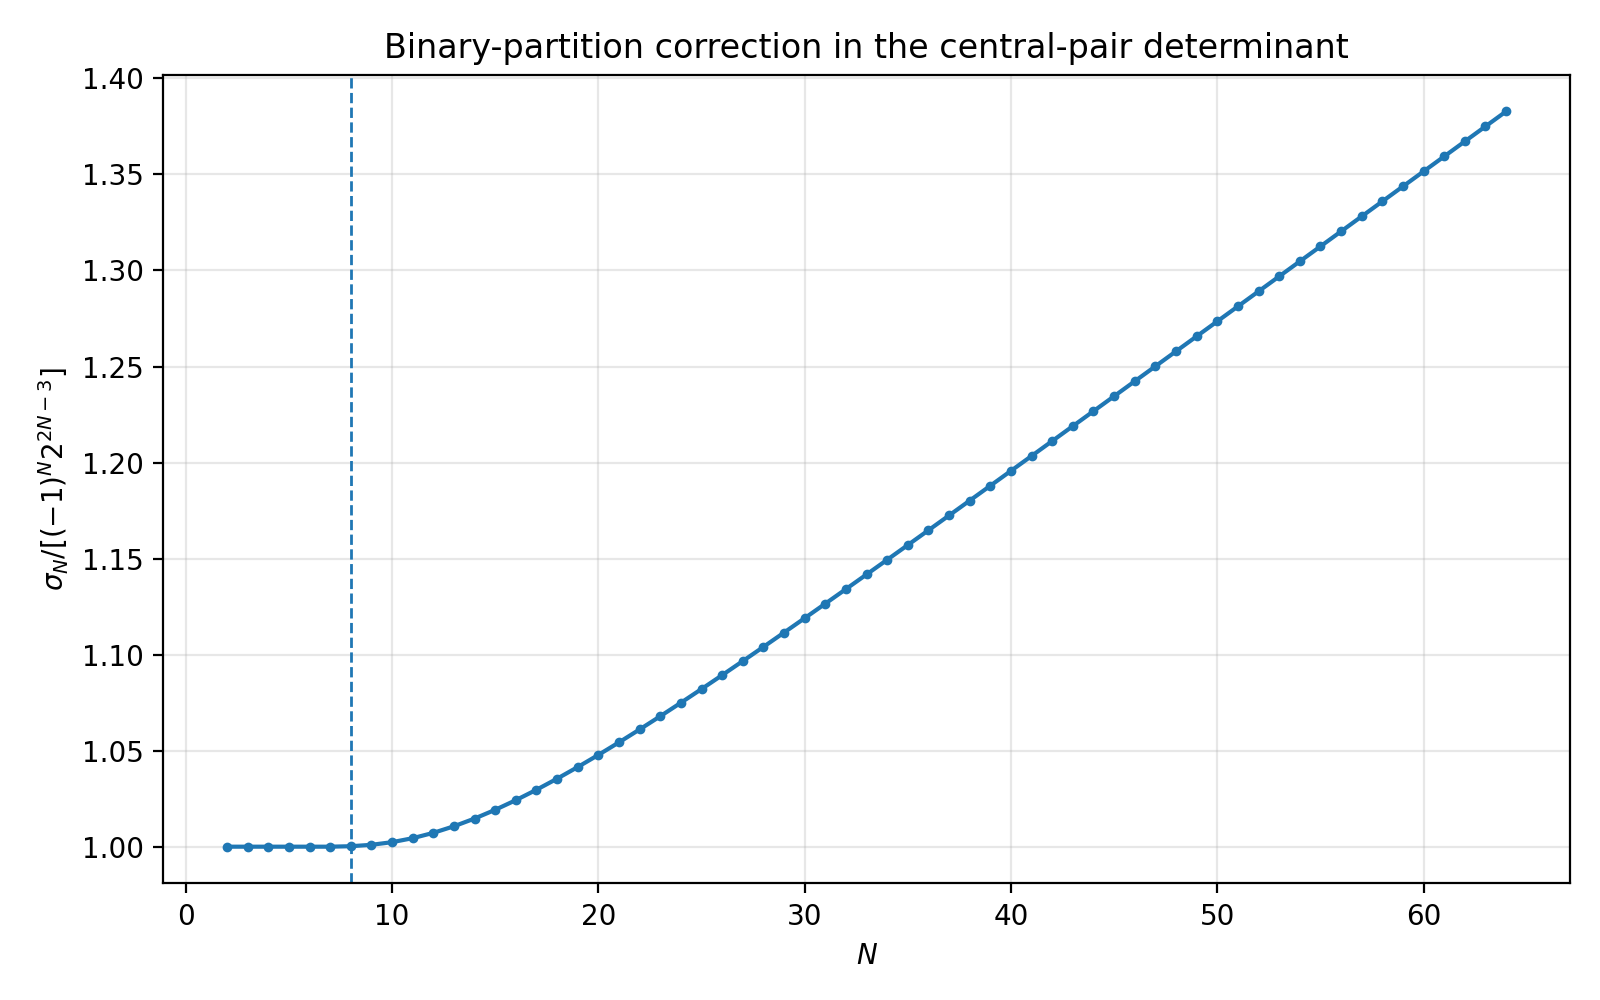
\includegraphics[width=0.88\textwidth]{sigma_binary_partition_ratio.png}
\caption{The normalized binary-partition correction $R_N$ through $N=64$.
The dashed line marks the first new dyadic part at $N=8$.}
\label{fig:sigma-ratio}
\end{figure}

Exact coefficient extraction verifies the alternating sign
$(-1)^N\sigma_N>0$ for every $2\le N\le128$.  This remains evidence rather
than proof for all $N$.

\subsection{Cancellation in exact central atomizations}

The central formulas are exact, but double precision rapidly loses digits as
the signed amplitudes grow.

\begin{table}[htbp]
\centering
\caption{Double-precision evaluation of exact central formulas for $P_{2N}$.}
\label{tab:roundoff}
\begin{tabular}{rrr}
\toprule
$N$ & largest raw pair amplitude & maximum reconstruction error\\
\midrule
1 & $9.47\times10^1$ & $9.22\times10^{-14}$\\
2 & $1.59\times10^5$ & $2.38\times10^{-10}$\\
3 & $2.94\times10^{10}$ & $4.21\times10^{-5}$\\
4 & $1.80\times10^{17}$ & $2.60\times10^{2}$\\
\bottomrule
\end{tabular}
\end{table}

\begin{figure}[htbp]
\centering
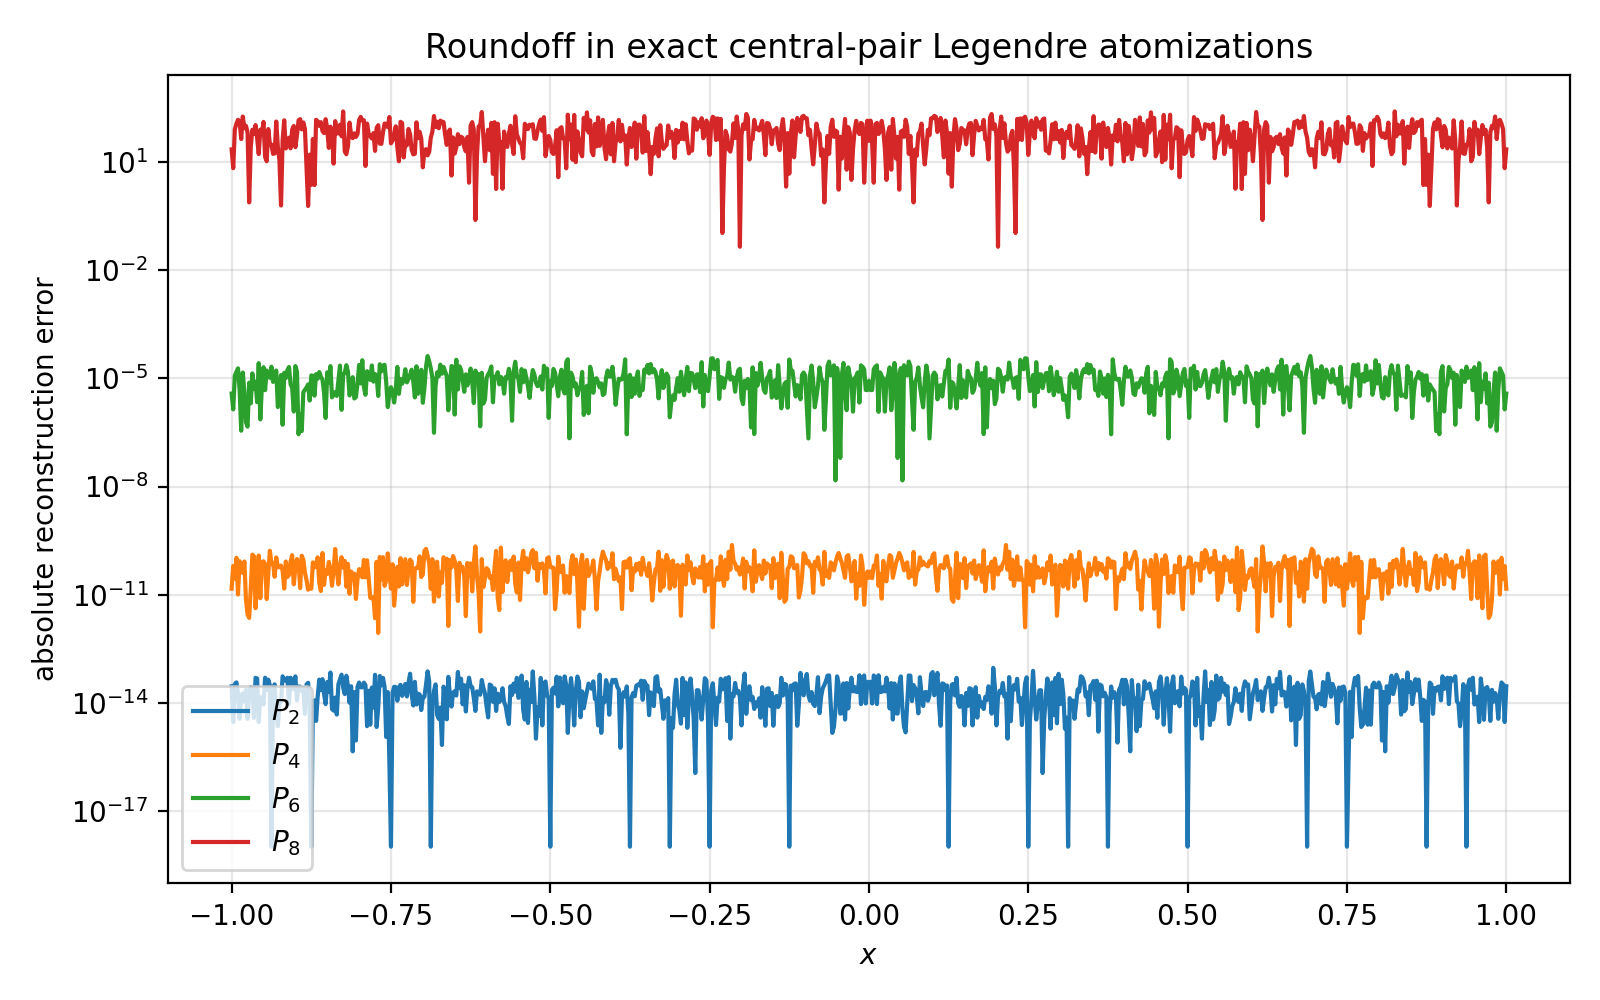
\includegraphics[width=0.92\textwidth]{central_pair_roundoff.png}
\caption{Pointwise floating residuals for exact central-pair representations.
The deterioration is cancellation in near-null Gram directions, not failure of
the identities.}
\label{fig:roundoff}
\end{figure}

The Gram identity \eqref{eq:energy-isometry} explains the phenomenon.  Stable
algorithms should preserve the Legendre blocks, use exact or multiprecision
arithmetic, or orthogonalize the atom coefficients in the $G$ metric before
evaluation.

\subsection{Legendre convergence}

\begin{figure}[htbp]
\centering
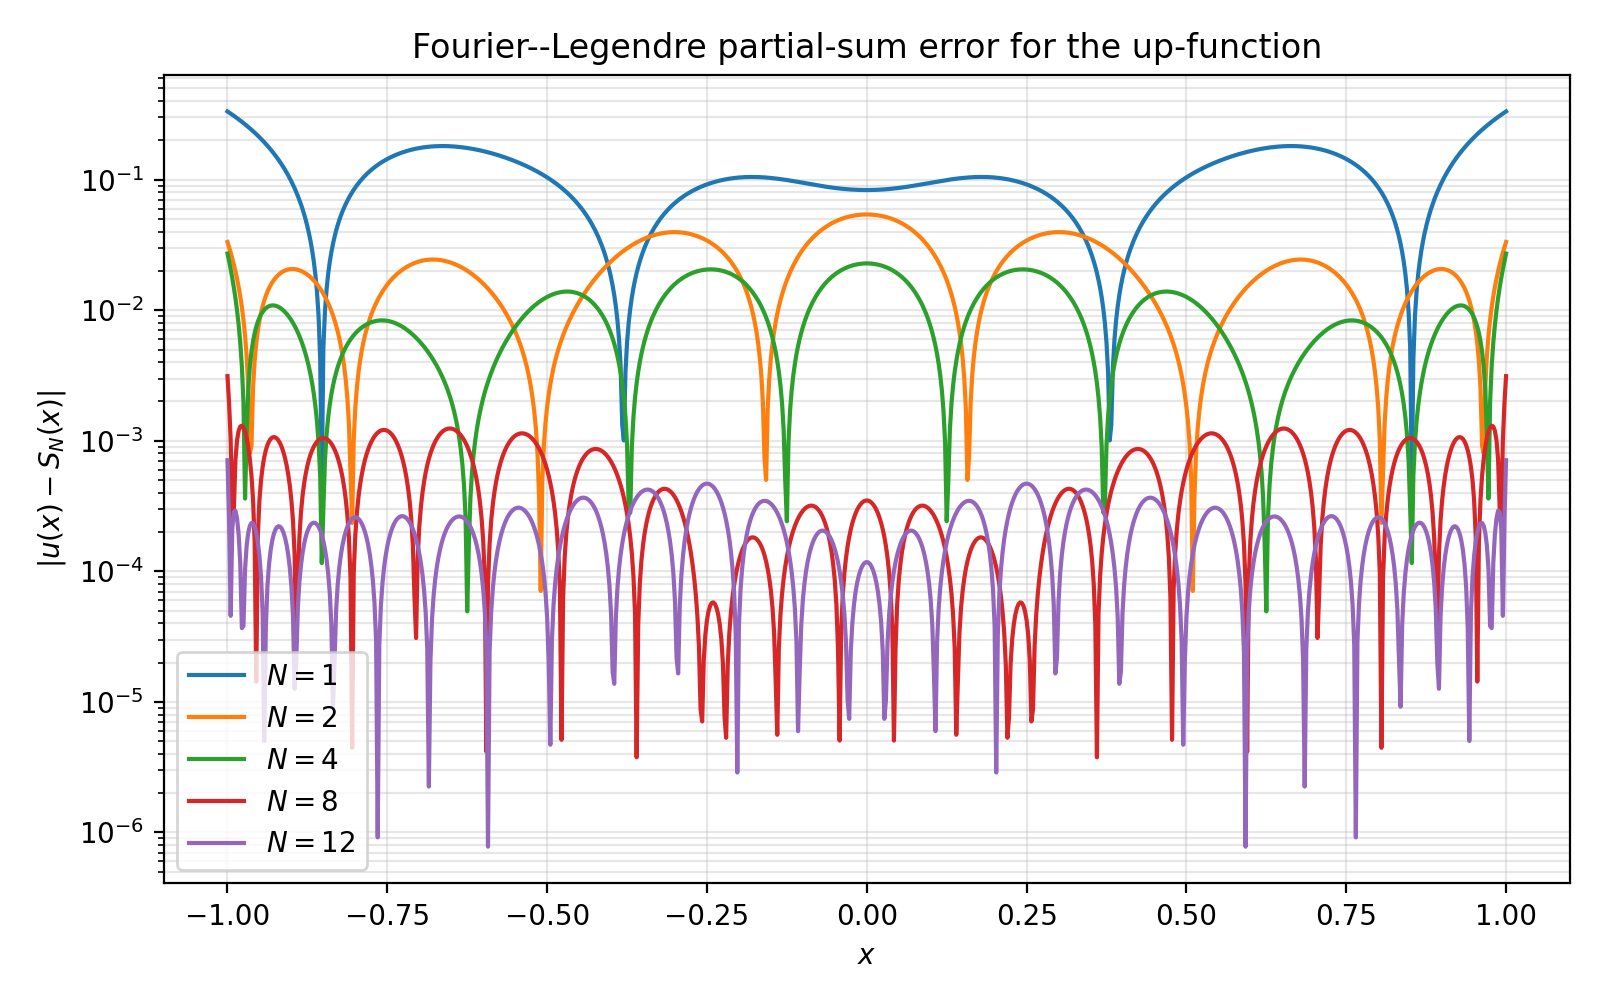
\includegraphics[width=0.92\textwidth]{legendre_partial_sum_error.png}
\caption{Error of the stable polynomial partial sum $S_N$.  The convergence is
superalgebraic but not necessarily monotone at each point or cutoff.}
\label{fig:legendre-error}
\end{figure}

The plotted curves use the polynomial side rather than raw central atoms.
Mathematically they are the same functions; numerically they inhabit very
different coordinate systems.

\subsection{An exact spectral transition at degree twelve}

The $Q_n$ are not a scalar orthogonal family, so real-rootedness is not
protected by Favard theory.  Exact Sturm counts in rational arithmetic give the
first transition.

\begin{proposition}[First nonreal zeros; exact computer-assisted certificate]
\label{prop:Q12-nonreal}
For $1\le n\le11$, $Q_n$ has exactly $n$ real roots.  The polynomial $Q_{12}$
has exactly eight real roots and therefore four nonreal roots.
\end{proposition}

\begin{proof}
The accompanying script constructs each $Q_n$ over $\mathbb Q$ and applies
Sturm's theorem.  For $Q_{12}$, the exact Sturm chain has degrees
$12,11,\ldots,0$ and leading-coefficient signs
\[
 +,+,+,+,+,+,+,+,-,+,+,+,+.
\]
At $+\infty$ this sequence has two sign variations.  At $-\infty$, parity of
the degrees gives
\[
 +,-,+,-,+,-,+,-,-,-,+,-,+,
\]
with ten variations.  Sturm's theorem therefore gives $10-2=8$ real roots.
The same exact calculation gives $n$ real roots for every $n\le11$.  The file
\texttt{Q12\_sturm\_certificate.txt} records the certificate and
\texttt{sturm\_real\_root\_counts.csv} records the complete table through
$n=20$.
\end{proof}

High-precision numerical roots locate the first conjugate quartet near
\begin{equation}
 \pm1.58181382985647\ \pm\ 0.189564695738147\,\ii.
 \label{eq:Q12-quartet}
\end{equation}
Exact nonreal-root counts for $n=12,\ldots,20$ are
\begin{equation}
 4,4,4,8,8,8,8,12,12.
 \label{eq:nonreal-counts}
\end{equation}

\begin{figure}[htbp]
\centering
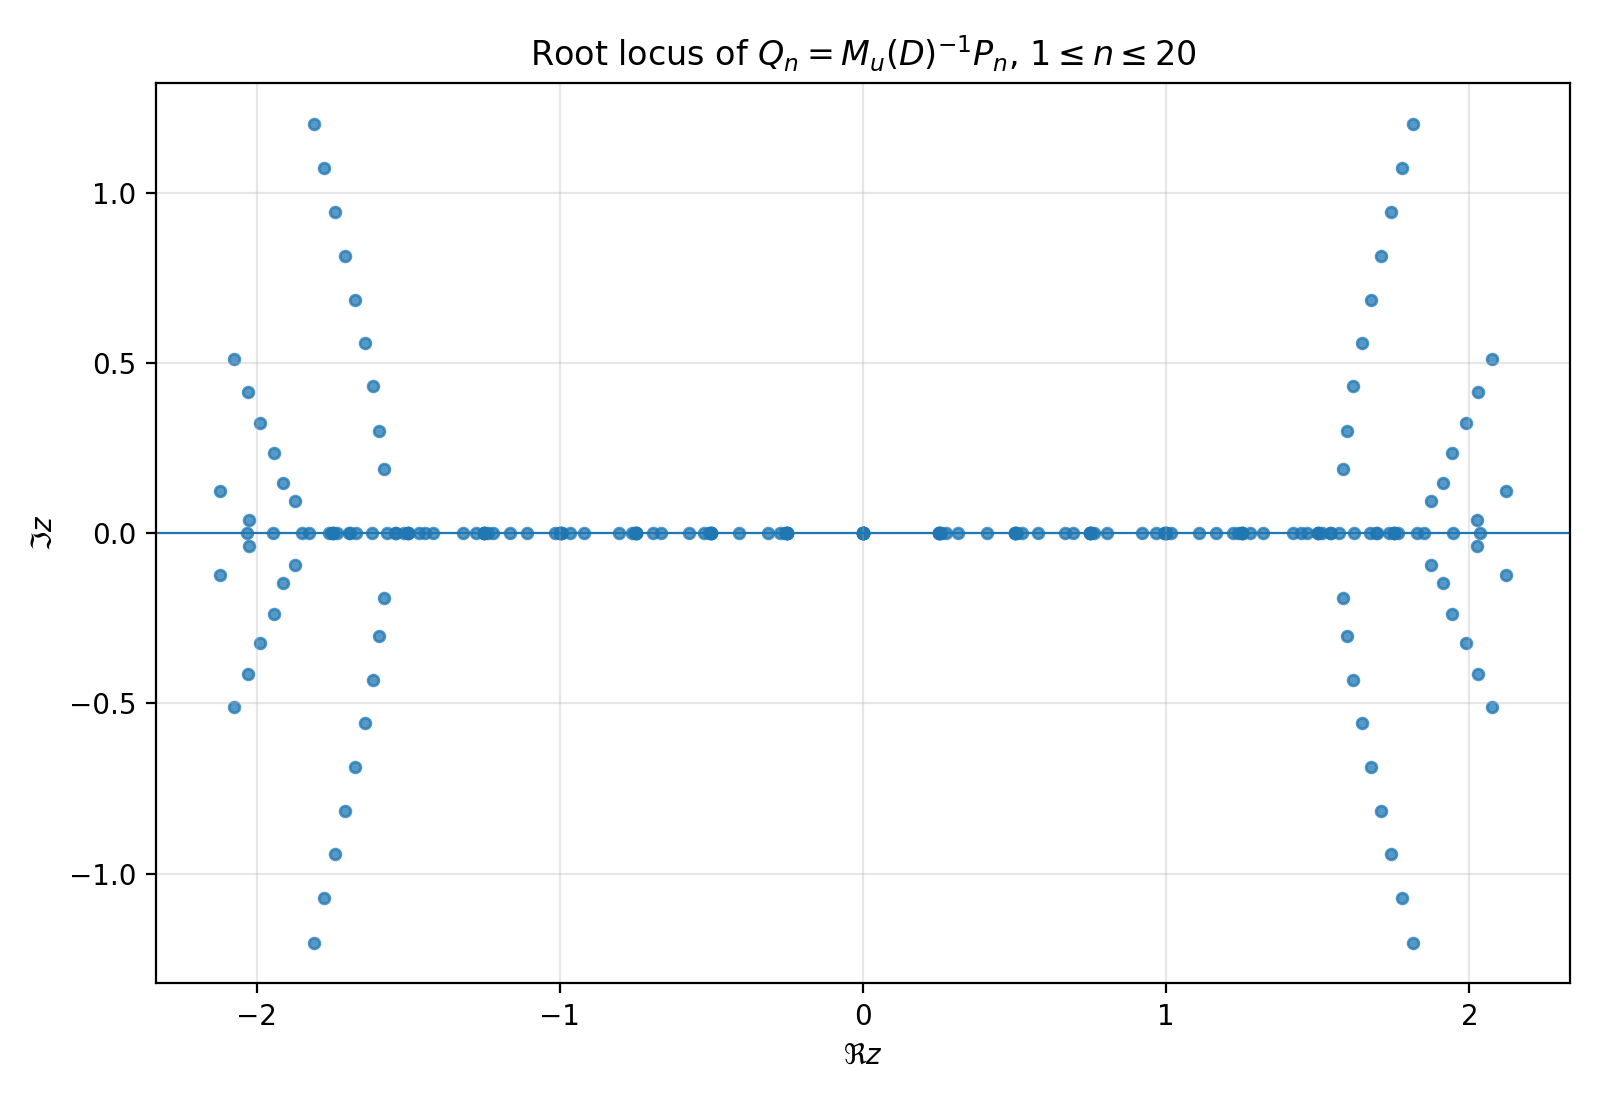
\includegraphics[width=0.88\textwidth]{deconvolved_legendre_root_locus.png}
\caption{Numerical root locus of $Q_n=\M(D)^{-1}P_n$ for $1\le n\le20$.
Real coefficients and parity force nonreal zeros into quartets.}
\label{fig:root-locus}
\end{figure}

This transition is consistent with the operator interpretation: $Q_n$ is
orthogonal in the pullback coordinate $X_u$, not under scalar multiplication by
$x$.

\section{Minimal central Gram geometry and structural interpretation}
\label{sec:interpretation}

The literal lattice is ideal for explicit sampling identities, while the
central basis is dimension-optimal for the even finite-dimensional space.  It
therefore has its own exact Gram and kernel calculus.

Define the physical central pair blocks
\begin{equation}
 \mathcal S_r^{(N)}(x)=\frac1M\left[
 u\!\left(\frac{x-(2r+1)}{2M}\right)
 +u\!\left(\frac{x+(2r+1)}{2M}\right)\right],
 \quad M=4^N,
 \label{eq:physical-central-pairs}
\end{equation}
and let $\mathbf S_N(x)$ be the column vector of these $N+1$ functions.  Write
\begin{equation*}
 \mathbf P_N(x):=(P_0(x),P_2(x),\ldots,P_{2N}(x))^{\mathsf T},
 \qquad C^{(N)}:=(c_{m,r}^{(N)}).
\end{equation*}
Then
\begin{equation}
 \mathbf P_N(x)=C^{(N)}\mathbf S_N(x).
 \label{eq:central-change-basis}
\end{equation}
Set
\begin{equation}
 \mathcal G_N=\int_{-1}^{1}\mathbf S_N(x)\mathbf S_N(x)^{\mathsf T}\dd x,
 \qquad H_N^+=\diag(h_0,h_2,\ldots,h_{2N}).
 \label{eq:central-Gram}
\end{equation}

\begin{theorem}[Central Gram factorization and dual basis; new]
\label{thm:central-Gram}
One has
\begin{equation}
 \boxed{
 C^{(N)}\mathcal G_N C^{(N)\mathsf T}=H_N^+,\qquad
 \mathcal G_N^{-1}=C^{(N)\mathsf T}(H_N^+)^{-1}C^{(N)}.}
 \label{eq:central-Gram-factorization}
\end{equation}
The $L^2$-dual functions to the central pairs are
\begin{equation}
 \eta_r^{(N)}(x)=\sum_{m=0}^{N}
 \frac{c_{m,r}^{(N)}}{h_{2m}}P_{2m}(x),
 \label{eq:central-dual}
\end{equation}
and satisfy
\begin{equation}
 \int_{-1}^{1}\eta_r^{(N)}(x)\mathcal S_s^{(N)}(x)\dd x=\delta_{rs}.
 \label{eq:central-dual-biorth}
\end{equation}
Finally, the even projection kernel has the pair-minimal factorization
\begin{equation}
 \boxed{
 K_N^+(x,y)=\mathbf S_N(x)^{\mathsf T}\mathcal G_N^{-1}\mathbf S_N(y).}
 \label{eq:minimal-kernel-factorization}
\end{equation}
\end{theorem}

\begin{proof}
Integrate \eqref{eq:central-change-basis} against its transpose and use
Legendre orthogonality.  Since $C^{(N)}$ is invertible, the inverse identity
follows.  In vector form, the proposed dual family is
$C^{(N)\mathsf T}(H_N^+)^{-1}\mathbf P_N
=\mathcal G_N^{-1}\mathbf S_N$; integrating against $\mathbf S_N$ gives the
identity matrix.  Finally,
\[
 K_N^+(x,y)=\mathbf P_N(x)^{\mathsf T}(H_N^+)^{-1}\mathbf P_N(y)
\]
and substitution of \eqref{eq:central-change-basis} gives
\eqref{eq:minimal-kernel-factorization}.
\end{proof}

This theorem compresses the two-sided factorization
\eqref{eq:two-sided-kernel} from $4M-1$ literal shifts in each variable to
$N+1$ reflection-pair blocks in each variable.  The price is that
$\mathcal G_N$ becomes severely ill-conditioned.

\subsection{Three exact coordinate systems}

At fixed cutoff $N$, the same polynomial $S_N$ has three exact descriptions:
\begin{enumerate}[leftmargin=1.8em,itemsep=0.25em]
\item the orthogonal Legendre coordinates $u_0,\ldots,u_N$, stable in
$L^2$ and spectrally natural;
\item the literal shift lattice, whose coefficients are sampled values of
$C_N=\Dscr S_N$ and whose redundancy exposes Poisson/sampling structure;
\item the central-pair coordinates $\alpha_N=C^{(N)\mathsf T}u$, which are
pair-count minimal and parity adapted but cancellation dominated.
\end{enumerate}
The coordinate transforms are exact; stability is not invariant under a
change of coordinates.  In particular, a huge determinant does not imply a
well-conditioned basis when the columns themselves have enormous norms and
nearly cancel.

\subsection{How the q-product enters}

The determinant mechanism has a clean hierarchy:
\[
 \text{dyadic zeros of }\widehat u
 \Longrightarrow \mathcal A_d(z)=\prod_{m\le d}[2^m]_z
 \Longrightarrow \mathcal A_d^{-1}
 \Longrightarrow \sigma_N
 \Longrightarrow \det\mathsf B_N.
\]
The Thue--Morse product controls the numerator side of dyadic cancellation,
while reciprocal $q$-integer products count restricted binary partitions.
The central basis therefore turns an analytic compact-support problem into an
integer coefficient-extraction problem.

\subsection{Why closure does not force analyticity}

Both \eqref{eq:block-loop} and \eqref{eq:symmetric-infinite-loop} express $u$
in terms of copies of itself, but neither is a finite-scale analytic
functional equation with uniformly summable scalar coefficients.  The literal
loop converges only after finite cancellation blocks are retained; the central
loop changes scale and coefficients with $N$.  These features are compatible
with the classical fact that the Fabius/up function is smooth but nowhere
analytic in the relevant sense.

\section{Conjectures and frontier problems}
\label{sec:frontiers}

The following statements are motivated by the exact formulas and computations,
but are not proved here.

\begin{conjecture}[Alternating sign of the central coefficient]
\label{conj:sigma-sign}
For every $N\ge2$,
\begin{equation}
 (-1)^N\sigma_N>0.
 \label{eq:sigma-sign-conj}
\end{equation}
\end{conjecture}

Exact computation verifies this for all $2\le N\le128$.  A proof may require
a sign-reversing involution for
\[
 [z^N](1-z)^{2N-2}\prod_{m\ge1}(1-z^{2^m})^{-1}
\]
or a contour argument adapted to the dyadic singularity set.

\begin{conjecture}[Subexponential binary-partition correction]
\label{conj:sigma-growth}
Let
\[
 R_N=\frac{(-1)^N\sigma_N}{2^{2N-3}}.
\]
Then $R_N\to\infty$ but
\begin{equation}
 \log R_N=o(N).
 \label{eq:sigma-subexp}
\end{equation}
Moreover, after subtraction of a smooth main term in $\log_2N$, the remainder
has a bounded log-periodic fluctuation characteristic of Mahler-type binary
partition products.
\end{conjecture}

The data through $N=128$ show positivity and slow growth, but are far too short
to distinguish competing asymptotic scales.  Mellin analysis of the reciprocal
$q$-product is a promising route.

\begin{conjecture}[Central Gram conditioning]
\label{conj:conditioning}
For the pair-minimal Gram matrix $\mathcal G_N$,
\begin{equation}
 \log\kappa_2(\mathcal G_N)=\Theta(N^2).
 \label{eq:conditioning-conj}
\end{equation}
Equivalently, pair-minimal central synthesis should have condition number
$\exp(\Theta(N^2))$.
\end{conjecture}

This is consistent with the $2^{\Theta(N^2)}$ arithmetic scales in
$C_N$ and the observed coefficient explosion, but determinant size alone is
not enough to prove it.  A proof should combine singular-value bounds for the
endpoint recurrence with the exact Gram factorization
\eqref{eq:central-Gram-factorization}.

\begin{conjecture}[Unbounded complex-zero population]
\label{conj:complex-zeros}
The number of nonreal zeros of $Q_n$ tends to infinity with $n$, and every
$Q_n$ has only simple zeros.
\end{conjecture}

The first nonreal quartet occurs exactly at degree $12$, and the exact counts
through degree $20$ are given in \eqref{eq:nonreal-counts}.  A natural program
is to study the eigenvalue problem for scalar multiplication $x$ in the
pullback-orthogonal basis, viewed as a nonnormal perturbation of the
self-adjoint $X_u$ recurrence.

\begin{problem}[Transmuted Christoffel asymptotics]
Determine the large-$d$ behavior of
\[
 \widetilde K_d(x,x)=\sum_{n=0}^{d}\frac{Q_n(x)^2}{h_n}
\]
in the bulk, at $x=0$, and near $\pm1$.  The factorial growth of deconvolution
suggests a scale very different from the classical Legendre Christoffel
function.  The operator identity \eqref{eq:operator-CD} should replace the
usual scalar quotient formula.
\end{problem}

\begin{problem}[Optimal symmetric pair placement]
Among all $N+1$ reflection pairs $\psi_k+\psi_{1-k}$ selected from the active
one-cell dictionary at degree $2N$, determine which choices minimize
$\kappa_2$ of the $L^2$ Gram matrix, the endpoint-coordinate matrix, or the
$L^\infty$ synthesis operator.  The central contiguous choice is arithmetically
canonical, but need not be numerically optimal.
\end{problem}

\begin{problem}[Stable evaluation and precision budgets]
Construct an algorithm that evaluates the central loops without expanding
near-null directions in ordinary Euclidean coordinates.  Candidates include
$G$-orthogonal QR, exact modular reconstruction, compensated pair summation,
and direct use of the dual basis \eqref{eq:central-dual}.  Balancing spectral
truncation error against coefficient amplification leads to implicit cutoff
relations of the type already treated by Lambert--$W$ asymptotics elsewhere in
the repository.
\end{problem}

\begin{problem}[Jacobi, Gegenbauer, and other symmetric bases]
For any symmetric polynomial family $R_n$ with a differential or
bispectral operator, define $\widetilde R_n=\Dscr R_n$.  The finite up-synthesis
and pullback orthogonality extend immediately, while conjugation transports the
spectral operator.  Work out explicit Jacobi/Gegenbauer analogues of
\eqref{eq:operator-CD}, determine their scalar-Favard obstructions, and compare
their central-pair conditioning.
\end{problem}

\begin{problem}[Beyond the dyadic atom]
For atomic functions generated by bases $a\ge3$ or by nonuniform product
scales, identify the analogues of $\mathcal A_d$, the parity split, and the
central determinant.  One expects reciprocal products related to restricted
$a$-ary partitions and generalized Thue--Morse/Prouhet sequences.  The dyadic
case suggests that determinant arithmetic may classify when symmetry-adapted
minimal dictionaries exist.
\end{problem}

\begin{problem}[Formal verification]
The central determinant proof is well suited to formalization: it reduces to a
palindromic recurrence, a truncated generating-function identity, a Toeplitz
row reduction, and integer parity.  A Lean development could import the
repository's existing Fabius/up infrastructure and certify the new basis,
determinant, Gram, and kernel identities independently of numerical evidence.
\end{problem}

\section{Conclusions}
\label{sec:conclusion}

The requested loop closes in its literal form by two exact transforms:
\[
 P_{2n}\xrightarrow{\ \Dscr\ \text{and sampling}\ }
 \text{finite shifted up-atoms},
 \qquad
 u\xrightarrow{\ \text{Legendre analysis}\ }(u_n)_{n\ge0}.
\]
Their composition is the blockwise self-representation
\eqref{eq:block-loop}.  The main analytical warning is that closure lives in
the grouped Legendre topology, not in an unconditional scalar atom series.

The new results sharpen this picture in three directions.  First, the
polynomials $Q_n=\Dscr P_n$ are ordinary Legendre polynomials viewed through a
nonlocal but positive pullback geometry.  Their true coordinate operator is
$X_u$, their spectral operator is $\Lscr$, and their Christoffel--Darboux
identity is operator valued.  The exact Favard obstruction and the first
nonreal zeros at degree $12$ show concretely why no scalar-weight theory can
replace this geometry.

Second, literal atom synthesis has an exact finite matrix calculus:
$D^{\mathsf T}GD=H$, $BD=I$, and the even projection kernel has a positive
rank-$(N+1)$ two-sided up-atom factorization.  These identities separate
functional exactness from Euclidean coefficient conditioning.

Third, reflection removes the one-dimensional nonpolynomial defect at every
even degree.  This creates a pair-minimal central basis, whose independence is
controlled by the odd integer determinant
$(-1)^N(C_N\sigma_N-1)$.  The determinant exposes a new bridge from the
Rvachev atom to reciprocal $q$-integer products and binary partitions.  It
also yields a symmetric common-scale loop for every Legendre partial sum,
converging superalgebraically in all derivatives.

The resulting picture is not merely a loop but a commuting network among
orthogonal polynomials, deconvolution Appell calculus, dyadic sampling,
$q$-products, parity quotients, and finite Gram geometry.  The most promising
next steps are the sign/asymptotic analysis of $\sigma_N$, stable central
coordinates, complex-zero asymptotics for $Q_n$, and formal verification.

\appendix

\section{Exact coefficient algorithms}
\label{app:algorithms}

This appendix records the recurrences used by the accompanying program.

\subsection{Moments and reciprocal-MGF coefficients}

Given cumulants $\kappa_r$, the complete Bell recurrences are
\begin{align}
 \mu_0&=1,&
 \mu_n&=\sum_{r=1}^{n}\binom{n-1}{r-1}\kappa_r\mu_{n-r},
 \label{eq:mu-recurrence}\\
 \gamma_0&=1,&
 \gamma_n&=-\sum_{r=1}^{n}\binom{n-1}{r-1}\kappa_r\gamma_{n-r}.
 \label{eq:gamma-recurrence}
\end{align}
These generate $\M$ and $1/\M$ in exact rational arithmetic.

\subsection{Deconvolved Legendre coefficients}

For a polynomial $p$ of degree $d$,
\begin{equation}
 \Dscr p=\sum_{j=0}^{d}\gamma_j\frac{p^{(j)}}{j!}.
 \label{eq:finite-deconv-algorithm}
\end{equation}
Equation \eqref{eq:Q-even-explicit} is the specialization to $P_{2n}$.

\subsection{Endpoint reduction}

Write $\mathcal A_d(z)=\sum_{j=0}^{R}a_jz^j$.  Given the first $R$ active
coefficients $n_0,\ldots,n_{R-1}$, extend by
\begin{equation}
 n_m=-\sum_{j=1}^{R}a_jn_{m-j},\qquad m\ge R,
 \label{eq:endpoint-forward-recurrence}
\end{equation}
using palindromicity to match the repository's shift convention.  Subtract the
resulting null sequence from the active vector; the final $d+2$ entries are the
endpoint coordinates.  The generating form is
\eqref{eq:endpoint-tail-gf}.

\subsection{Binary-partition coefficient}

Let $p_j$ be the coefficients of
\begin{equation}
 \prod_{m\ge1}(1-z^{2^m})^{-1}=\sum_{j\ge0}p_jz^j.
 \label{eq:binary-partition-gf}
\end{equation}
They are computed by the unbounded-coin recurrence for parts
$2,4,8,\ldots$.  Then
\begin{equation}
 \sigma_N=\sum_{j=0}^{N}(-1)^j\binom{2N-2}{j}p_{N-j}.
 \label{eq:sigma-convolution}
\end{equation}
Only powers of two not exceeding $N$ are required.

\subsection{Central coefficients}

For fixed $N$, form the endpoint-coordinate matrix of the pairs
$S_r^{(N)}$.  Solve the nonsingular $(N+1)\times(N+1)$ minor for each target
$P_{2m}(2t-1)$.  The program then verifies all remaining endpoint rows exactly.
The closed-loop vector is
\begin{equation}
 \alpha_N=C^{(N)\mathsf T}(u_0,\ldots,u_N)^{\mathsf T}.
 \label{eq:alpha-matrix}
\end{equation}

\section{Reproducibility inventory}
\label{app:reproducibility}

The archive accompanying this report contains:
\begin{description}[leftmargin=3.6cm,style=nextline]
\item[\texttt{legendre\_rvachev\_closed\_loop.tex}]
The complete LaTeX source.
\item[\texttt{legendre\_rvachev\_closed\_loop.pdf}]
The rendered report.
\item[\texttt{legendre\_up\_experiments.py}]
Fully commented exact and numerical experiment code.
\item[\texttt{numerical\_results.txt}]
Human-readable exact values and diagnostics.
\item[CSV tables]
Exact central coefficients, closed-loop coefficients, determinant checks,
$\sigma_N$ data, Legendre coefficients, Sturm counts, roots, and floating
errors.
\item[PNG figures]
The determinant correction, roundoff, Legendre convergence, and root locus
figures used in the report.
\item[\texttt{Q12\_sturm\_certificate.txt}]
The exact degree/sign certificate used in \cref{prop:Q12-nonreal}.
\end{description}

The calculations can be regenerated with
\begin{lstlisting}[style=pythonstyle]
python legendre_up_experiments.py
\end{lstlisting}
The report can then be compiled with a standard modern LaTeX installation.
All exact claims in the numerical section are independent of Fourier
truncation; only the plotted function values use floating arithmetic.

\begin{thebibliography}{99}

\bibitem{Fabius1966}
J. Fabius,
\emph{A probabilistic example of a nowhere analytic $C^\infty$-function},
Zeitschrift f\"ur Wahrscheinlichkeitstheorie und Verwandte Gebiete
\textbf{5} (1966), 173--174.

\bibitem{Szego}
G. Szeg\H{o},
\emph{Orthogonal Polynomials},
4th ed., American Mathematical Society Colloquium Publications, Vol.~23,
American Mathematical Society, 1975.

\bibitem{Roman}
S. Roman,
\emph{The Umbral Calculus},
Academic Press, 1984.

\bibitem{Comtet}
L. Comtet,
\emph{Advanced Combinatorics},
D. Reidel, 1974.

\bibitem{ReshetnikovPrimary}
V. Reshetnikov,
\emph{The Fabius Function and Rvachev's Up-Function},
primary exposition in the ProveIt repository,
\url{https://github.com/VladimirReshetnikov/ProveIt/blob/main/Analysis/FabiusFunction/docs/Fabius_Function_and_Rvachev_Up.tex},
accessed 29 August 2026.

\bibitem{ReshetnikovSynthesis}
V. Reshetnikov,
\emph{Up Polynomial Synthesis},
consolidated polynomial-reproduction volume in the ProveIt repository,
\url{https://github.com/VladimirReshetnikov/ProveIt/blob/main/Analysis/FabiusFunction/docs/Up_Polynomial_Synthesis.tex},
accessed 29 August 2026.

\bibitem{ReshetnikovLoopV3}
V. Reshetnikov,
\emph{Closing the Lagrange--Legendre--Rvachev Loop},
repository draft \texttt{lagrange\_rvachev\_loop.tex}, in the recursive
\texttt{Analysis/FabiusFunction/docs} tree,
\url{https://github.com/VladimirReshetnikov/ProveIt/tree/main/Analysis/FabiusFunction/docs},
accessed 29 August 2026.

\bibitem{ReshetnikovLoopV4}
V. Reshetnikov,
\emph{Lagrange--Rvachev Closed-Loop Report},
repository draft \texttt{lagrange\_up\_loop.tex}, in the recursive
\texttt{Analysis/FabiusFunction/docs} tree,
\url{https://github.com/VladimirReshetnikov/ProveIt/tree/main/Analysis/FabiusFunction/docs},
accessed 29 August 2026.

\bibitem{ProveItManifest}
V. Reshetnikov,
\emph{Fabius-function documentation manifest and provenance maps},
ProveIt repository,
\url{https://github.com/VladimirReshetnikov/ProveIt/tree/main/Analysis/FabiusFunction/docs},
accessed 29 August 2026.

\end{thebibliography}

\end{document}
